\section{Foundations}
\label{sec:Foundations}

\NOTE{\emph{Length:} 2 p., \emph{Responsible:} Tony}
\NOTE{Based on BX 2017 paper, Section~3.1. Should include the taxonomy of Figure~3.}

In this section, we introduce the basic terms required in the rest of the paper to describe and discuss the different bx approaches and solutions to our benchmark.
We first of all define the \emph{input and output data} for bx tools in Section~\ref{sec:io-data}.
Based on this, we identify two \emph{basic operations} applied by bx tools to restore consistency in Section~\ref{sec:basicOperations}.
This finally allows us to describe and discuss a series of possible bx tool architectures in Section~\ref{sec:bx-tool-architectures}.
For each solution and bx tool presented in Section~\ref{sec:Solutions}, we assign the best fitting architecture as a means of abstracting from technical details and focusing on the conceptual core strategy applied by each tool.   

\subsection{Input and Output Data}
\label{sec:io-data}

We refer to the input and output data expected and produced by a bx tool as \emph{models} and \emph{deltas}, representing the data to be kept consistent, and changes applied to models, respectively.  

\begin{definition}[Model]~\\
\label{def: model}
\emph{A model, denoted by capital (primed) letters $A$, $A'$, $B$, $B'$, is a generic term used to refer to the data to be kept consistent by a bx tool.}
\end{definition}
%
We view the concrete representation of a model, e.g., as a graph, a tree, a set, as being \emph{internal} to a bx tool and is not of primary relevance (for the goals and scope of this paper).
Note that (double, triple) primed letters such as $A$, $A'$ indicate that these models are somehow related.

\begin{example}[Models]~\\
An example of two models from the Families-to-Persons case is depicted in Figure~\ref{fig:models}.
The internal structure of these models is represented using typed, attributed graphs.
\end{example}

\begin{definition}[Delta]~\\
\label{def: delta}
\emph{A delta, denoted by an arrow $\delta: A \rightarrow A'$ going from a ``before'' to an ``after'' model, is a generic term used to refer to the relation between two models, where these models are to be interpreted as being two versions (before and after) of the same model.}
\end{definition}
%
Again the concrete representation of a delta, e.g., as a span of mappings or as a change log, is internal to a bx tool and is not of primary relevance.
In order to precisely classify our tests in the benchmark, however, we distinguish between delta representations that record the \emph{order} in which changes were made, and delta representations that only provide a structural mapping between two versions of a model:  

\begin{definition}[Operational Delta, o-delta]~\\
\label{def: o-delta}
\emph{An operational delta, denoted by $(\delta): A \stackrel{@}{\rightarrow} A'$, is a delta that represents the changes made to a model as an ordered sequence of applied change operations.}
\end{definition}
%
While the exact set of available change operations may vary depending on the chosen technological space, we assume the following set of change operations, which is typical in an MDE (graph-based) setting:  (i)~addition of elements (objects and links in a model), (ii)~deletion of elements, (iii)~attribute changes, and (iv)~movement of objects.
Note that our interpretation of ``movement'' corresponds to a change of the container relation (as defined by Ecore) of an object.

\begin{definition}[Structural Delta, s-delta]~\\
\label{def: s-delta}
\emph{A structural delta, denoted by $\langle\delta\rangle: A \Rightarrow A'$, is a delta that represents the changes made to a model as a purely structural mapping between the model and the version of the model after applying the changes.}
\end{definition}
%
As it is impossible to discern from an s-delta $\langle\delta\rangle$ the exact order in which change operations were applied, it can be represented as various, in this sense equivalent o-deltas $(\delta), (\delta'), ...$.

Finally, test cases in the benchmark are implemented as a series of model \emph{edits}, representing changes \emph{to be applied}.
It is helpful for conceptual clarity to differentiate edits from deltas.
Edits can produce deltas when applied to models, but can also fail:

\begin{definition}[Edit]~\\
\label{def: edit}
\emph{An edit, denoted by $@: M \rightarrow \Delta$ is a partial function $@$ from a set of models $M$ to a set of deltas $\Delta$.
If an edit is applicable to a model $@$, it can be applied to yield a delta $\delta$, i.e., 
$@: A \longmapsto \delta: A \rightarrow A'$}.
\end{definition}

\begin{example}[Deltas and Edits]~\\
Given the persons model to the right of Figure~\ref{fig:models}, an s-delta would be:
\begin{quote}
\emph{Added two female persons \texttt{(Anne, Miller)} and \texttt{(Sandra, Miller)}} to the persons register.
\end{quote}
Representing the same change as an o-delta requires fixing the order in which these female persons were added to the person register, for instance:
\begin{quote}
\emph{Added two female persons to the register in the order \texttt{[(Anne, Miller), (Sandra, Miller)]}}.
\end{quote}
As explained in Section~\ref{sec:FamiliesToPersons}, this distinction is required to pass some of the tests in the benchmark.
In contrast, an edit would be, for example:
\begin{quote}
\emph{Attempt to delete the female person \texttt{(Anne, Miller)} from the register}.    
\end{quote}
This edit is not applicable to the register depicted to the right of Figure~\ref{fig:models}, but would be applicable to the resulting register referenced by the deltas above.  
\end{example}

Models and deltas are typically grouped into \emph{domains} or \emph{kinds}.
We use the term model space to refer to this grouping:
%
\begin{definition}[Model Space]~\\
\label{def: model-space}
\emph{A model space, denoted by $\mathcal{M} = (\Delta, M)$, consists of a set of deltas $\Delta$ between models taken from a set of models $M$. 
In the binary case, we denote one of the model spaces as the source model space: $\mathcal{M}_S = (\Delta_S, M_S)$, and the other as the target model space:  $\mathcal{M}_T = (\Delta_T, M_T)$.}
\end{definition}

While deltas represent relations between models in the same model space, \emph{correspondences} represent relations between models in different model spaces:
\begin{definition}[Correspondence, corr]~\\
\label{def: corr}
\emph{A correspondence (or just corr), denoted by a bidirectional arrow $\sigma : A \leftrightarrow$ B, refers to a relation between two models typically in different model spaces.}
\end{definition}

In order to support an intuitive understanding of the diagrams used to discuss the tool architectures in Section~\ref{sec:basicOperations}, deltas are often depicted visually as \emph{vertical} single-headed arrows, while corrs are depicted visually as \emph{horizontal} double-headed arrows.
The models connected by a corr are typically interpreted as being in the same version, with respect to the relevant deltas being discussed.
In many cases, it is conceptually helpful to regard some correspondences as being \emph{diagonal} in the sense that they represent correspondences between models (in different model spaces) that are in different versions with respect to the relevant deltas being discussed: 
\begin{definition}[Diagonal, diag]~\\
\label{def: diag}
\emph{A diagonal (or just diag), denoted by $\sigma : A' \leftrightarrow$ B, is a corr that is ``diagonal'' in the sense that it connects two models in different versions ($A'$ is in an updated, new version, while $B$ is in an old version) with respect to a set of deltas being discussed.} 
\end{definition}

While arbitrary pairs of models can be connected in some way or another with a corr (or diag), not all corrs make sense for a given consistency management scenario.
This is expressed by assuming an underlying \emph{consistency relation} that can be used to classify corrs as being either consistent or not.
This is summarized together with all previous definitions in the following:
\begin{definition}[Triple Space]~\\
\emph{A triple space, denoted by the triple $(\mathcal{M}_S, \mathcal{M}_T, C \subseteq R)$, consists of a source model space $\mathcal{M}_S$, a target model space $\mathcal{M}_T$, a set of corrs $R$ connecting models in the source and target model spaces, and a consistent subset of corrs $C \subseteq R$.
A corr $c \in R$ is said to be consistent if and only if $c \in C$.}
\end{definition}

\begin{remark}[Formalization]~\\
Model spaces can be formalized as \emph{categories} with models as objects and deltas as arrows.
If deltas are formalized as spans of structure-preserving mappings, then delta composition can be formalized as a pullback of spans.
Similarly to deltas, corrs and diags can also be formalized as spans of structure-preserving mappings.
The interested reader is referred to e.g., Anjorin~\cite{DBLP:conf/ac/Anjorin16}, or Diskin et al.~\cite{JOT:issue_2011_01/article6} for further details.
\end{remark}

\begin{example}[Model Spaces, Corrs, and Triple Space]~\\
The source (target) model space for the Families-to-Persons case consists of all models that are valid instances of the families (persons) metamodel depicted to the left (right) of Figure~\ref{fig:metamodels}, and all deltas between the models in each model space representing all possible combinations of the basic change operations (add/delete elements, attribute changes, object movements).

For the Families-to-Persons case, corrs can be represented by bijective mappings between family members and persons.
Consistent corrs additionally satisfy the two constraints given in Section~\ref{sec:MetamodelsAndConsistency}.  
For the pair of models depicted in Figure~\ref{fig:models}, for example, a \emph{consistent} corr would consist of mappings $fm\langle n \rangle \leftrightarrow p\langle n \rangle$ for $n \in \{1, ..., 6 \}$.

The resulting triple space for the benchmark consists of these two model spaces, the set $R$ of all possible corrs (bijections between family members and persons), and the consistent subset $C \in R$ of corrs that satisfy the two additional constraints. 
\end{example}

We use triple spaces to abstract from exactly how the underlying consistency relation is specified or checked by concrete bx tools.
To achieve a high-level but still useful abstraction for \emph{consistency management} strategies, we now discuss a few basic consistency management operations in the following. 


\subsection{Basic Operations}
\label{sec:basicOperations}

While we do not aim to describe and discuss in detail exactly how bx tools internally manage consistency, we claim that there is actually only a small set of basic operations, which are applied and combined in different ways to realize different bx tool \emph{architectures}.
These architectures can be used to classify bx tools and characterize fundamental differences and similarities.

% Groups of operations
% Notation in Fig. 3
Figure~\ref{fig:basicOperationsOverview} provides an overview of five basic operations showing their arity and indicating input and output parameters.
Using the same notation as for Definitions~\ref{def: model}, \ref{def: delta}, and \ref{def: corr}, models are depicted as (primed) capital letters, deltas as vertical single-headed arrows, and corrs (diags) as horizontal (diagonal) double-headed arrows.
The five operations are depicted as rectangles, connected to their input via incoming, and to their output via outgoing dotted single-headed arrows. 
These operations are now explained in the following by providing concrete examples taken from our Families-to-Persons benchmark:

\begin{figure}[bt!]
	\centering
	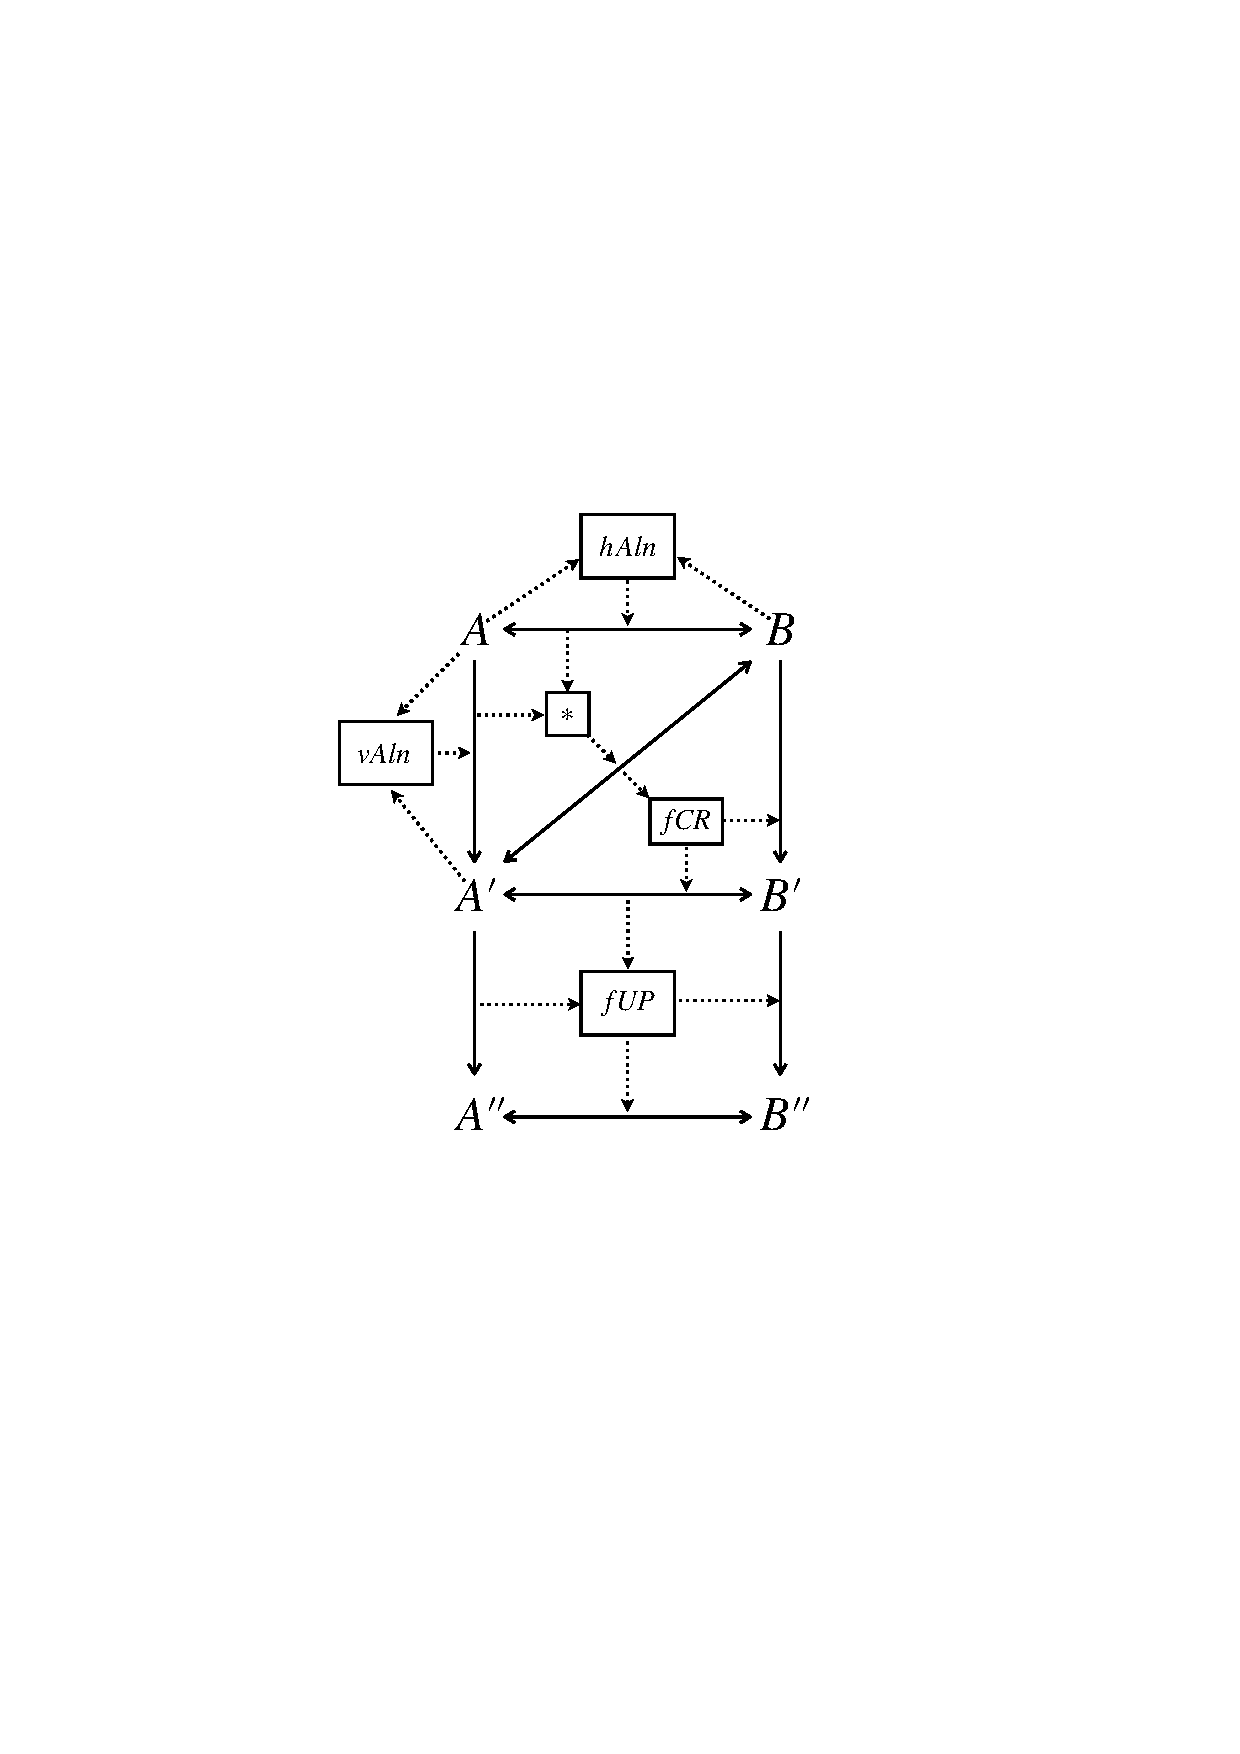
\includegraphics[width=0.55\columnwidth]{diagrams/foundations//BasicOperationsOverview}
	\caption{Overview of basic operations}
	\label{fig:basicOperationsOverview}
\end{figure}

% Explanation
\begin{description}
\item[\emph{Horizontal Alignment (hAln)}] takes two models $A$ and $B$ in different model spaces and determines a corr $A \leftrightarrow B$ between them. 
It is in general impossible to recover unique corrs and $hAln$ is often heuristic-based.
For the Families-to-Persons case, a simple strategy would be to pair female(male) persons and family members with the right gender and same family name and name according to convention.
The pair of models depicted in Figure~\ref{fig:models}, however, shows that this is not sufficient to obtain \emph{the} unique correspondence when there are multiple persons with the same name in the person register.

\item[\emph{Vertical Alignment (vAln)}] takes two models $A$ and $A'$ in the same model space and determines a delta $A \rightarrow A'$.
This is also non-deterministic in general as there can be multiple deltas going from $A$ to $A'$.
Consider, for example, renaming a person \texttt{Smith, Mary} to \texttt{Smith, Anne}, as opposed to deleting \texttt{Smith, Mary} and adding a new person \texttt{Smith, Anne} with the same birthday.
It is impossible to decide what \emph{the} delta is in this case, and $vAln$ must apply suitable heuristics to make a choice. 

\item[\emph{Re-Alignment ($\ast$)}] takes a coinciding corr and delta and produces a diag by combining them.  
The idea is that two models $A$ and $B$ were previously aligned via $A\leftrightarrow B$.
The $A$ was changed to $A'$ yielding the delta $A \rightarrow A'$.
The task of $\ast$ is now to ``re-align'' the new $A'$ with $B$.
Re-alignment is often a straightforward task of updating the corr, removing obsolete (invalid) mappings due to deleted (changed) elements in $A$, as well as adding any new mappings from added (changed) elements in $A$ to existing elements in $B$.
Although we introduce $\ast$ as depicted in Figure~\ref{fig:basicOperationsOverview}, we shall also use variants of $\ast$ with different input/output roles for the parameters, e.g., taking the diag as input and producing corr and delta as output.
For simplicity, we shall also refer to these operations as re-alignment, indicating clearly in the diagrams which parameters are taken as input and which are produced as output.

\item[\emph{Forward Consistency Restoration (fCR)}] takes as input a diag $A' \leftrightarrow B$ and determines a delta $B \rightarrow B'$ and a \emph{consistent} corr $A' \leftrightarrow B'$.
This operation obviously requires some knowledge of the underlying consistency relation.
The input diag is typically not yet consistent and some strategy of how to restore consistency by changing $B$ in some appropriate manner must be implemented.
For example, if an unmapped family member in $A'$ and an unmapped person in $B$ are found, a strategy to restore consistency would be to rename the person in $B'$ so that a consistent corr can be reestablished.
Consistency restoration (backward consistency restoration ($bCR)$ is defined analogously) is often non-deterministic, hence the need for laws to characterize ``desirable'' behaviour.

\item[\emph{Forward Update Propagation (fUP)}] takes a different approach to consistency maintenance than $fCR$.
Instead of restoring consistency to an already inconsistent diag, $fUP$ takes as input a (typically consistent) corr $A' \leftrightarrow B'$ and a delta $A' \rightarrow A''$.
To decide how to maintain consistency, $fUP$ inspects the input delta $A' \rightarrow A''$ and \emph{propagates} the delta to $B'$, yielding an output delta $B' \rightarrow B''$ as well as a consistent corr $A'' \leftrightarrow B''$.
For example, adding a new family member to $A'$ to yield $A''$ can be propagated to adding a suitably named new person to $B'$ to yield $B''$, and adding a mapping between the new family member and person in $A'' \leftrightarrow B''$.  
Similar to consistency restoration, update propagation (backward update propagation ($bUP)$ is defined analogously) is also often non-deterministic.
\end{description}

\subsection{Input-Based Application Scenarios}
\label{sec:application-scenarios}

In this section, we now discuss 11 different application scenarios according to the provided input data in each case.
If certain input data, e.g., the input delta, is available or not is often an intrinsic part of an application scenario.
Consider, for example, an application scenario in which models are manipulated without any means of tracking exactly what changes were made.
If this is part of the requirements (perhaps due to an existing process workflow at a company) and cannot be influenced, then input deltas will not be available for consistency management.
%
To classify all possible application scenarios Figure~\ref{fig:architectureLandscape} depicts a grid distinguishing horizontal and vertical input data to yield 11 possible combinations.

The possibilities for vertical input data range from just the changed source model $A'$ (initial-), to the old and changed source models $A$, $A'$ (state-), to the input delta $A \rightarrow A'$ (delta-).
While the terms \emph{state} and \emph{delta} should be natural, \emph{initial} deserves some explanation.
If a bx tool is supplied the changed model $A'$ as vertical input, it can only reasonably assume that the implied input delta is $\emptyset \rightarrow A'$, i.e., the model $A'$ has been created from scratch (even if this is not the case).
The empty model $\emptyset$ is often referred to as the \emph{initial object} and the unique existence of $\emptyset \rightarrow A'$ is required.

\begin{figure}[tb!]
	\centering
	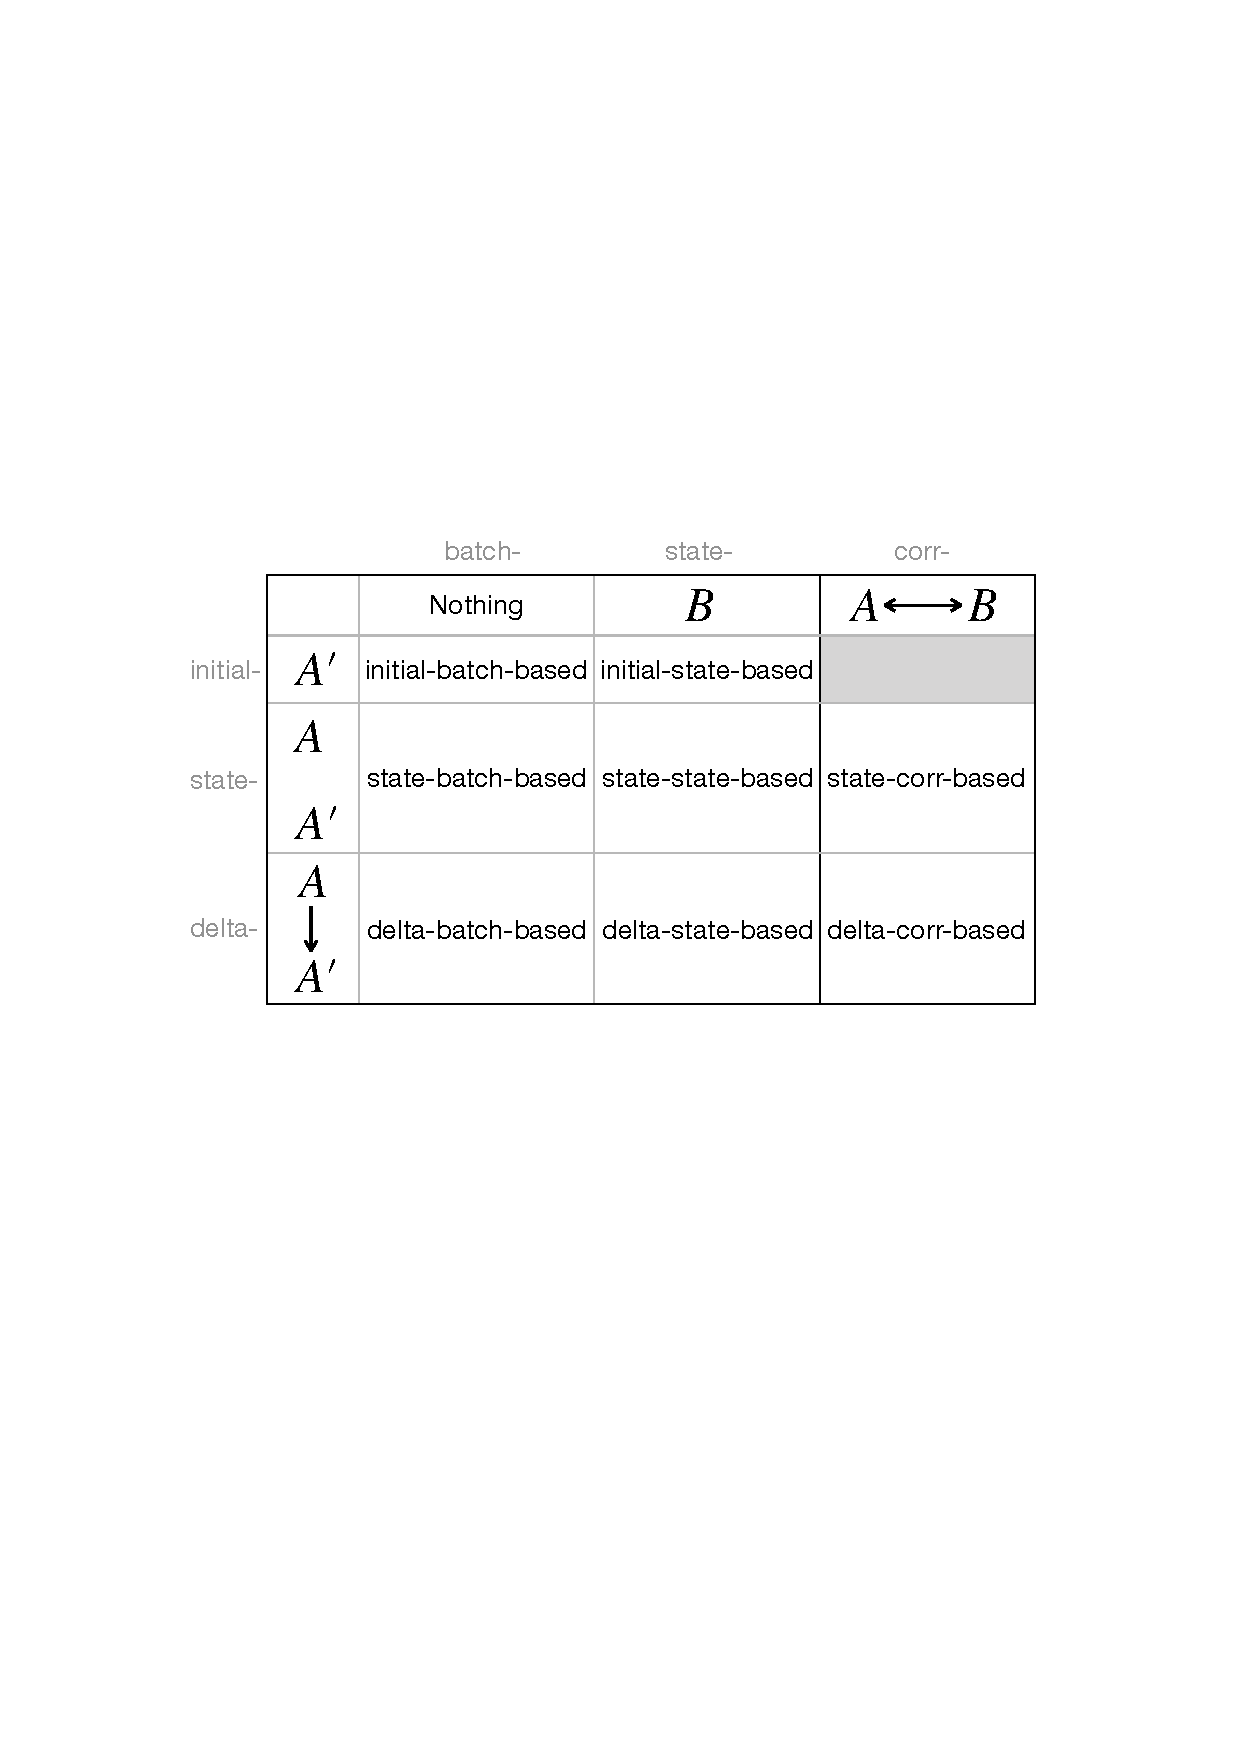
\includegraphics[width=0.9\columnwidth]{diagrams/foundations//ArchitectureLandscape}
	\caption{Overview of bx application scenarios}
	\label{fig:architectureLandscape}
\end{figure}

The possibilities for horizontal input data range from nothing (batch-), to just the previous target model $B$ (state-), to the corr between previous source and target models $A \leftrightarrow B$, to the diag between the changed source model and previous target model $A' \leftrightarrow B$.
All combinations of vertical and horizontal input are theoretically possible, apart from initial-corr-based, which would be identical with state-corr-based and is therefore omitted.
Compared to the commonly used but imprecise terms \emph{state-based} or \emph{delta-based}, our classification schema allows for a fine-granular distinction between, e.g., \emph{state-state-based} and \emph{delta-state-based}, etc.

From an inspection of all bx tools we are aware of, it is our observation that tool architectures tend to be either restoration-based (i.e., using basic operations \emph{fCR}, \emph{bCR}) or propagation-based (i.e., using basic operations \emph{fUP} and \emph{bUP}), but not both.
A plausible explanation is that implementing both \emph{fCR} and \emph{fUP} would be redundant as both serve the same purpose of consistency maintenance.
All other basic operations are more auxiliary in nature and help compensate a mismatch between application scenario and tool architecture.

Such a mismatch stems from the fact that bx tool developers choose a certain bx tool architecture corresponding to one of the 11 application scenarios, i.e., to their expectations concerning what input data is available and what not.
If a bx tool expects more input data than is available, it can only be used in combination with external alignment operations, which are required to recover the missing data.
This situation can be problematic as apriori alignment can be imprecise, inefficient, and difficult to implement.
Faced with this overfitting mismatch, users of such a bx tool tend to view the tool as being heavy-weight, having unrealistic (utopic) expectations, and thus not being worth the effort if one has to implement all required additional auxiliary alignment operations.

If a bx tool requires less input data than is available, the additional input data is simply ignored.
While the required alignment is either completely internalized, e.g., via the use of in-built heuristics and optimization, or is well-supported with an appropriate language or API, our benchmark shows that this situation is still undesirable as it leads to unexpected results in general.
Faced with this underfitting mismatch, users of such a bx tool tend to view the tool as being a lightweight, but often unpredictable, unconfigurable black-box.

As realizing which underlying architecture a bx tool implements is crucial for understanding its limitations and strengths/weaknesses (in comparison with other bx tools with different underlying architectures), we discuss in the following possible restoration-based and propagation-based tool architectures for each of our 11 identified application scenarios. 

\subsection{BX Tool Architectures}
\label{sec:bx-tool-architectures}

Figure~\ref{fig:initialBatchBased} depicts bx tool architectures for the simplest application scenario, namely \emph{initial-batch-based}.
As this application scenario can actually be handled with a standard unidirectional model transformation, the architectures are not necessarily practical, but simply show how a bx tool can easily handle simple cases as degenerate versions of the more general case of consistency maintenance.
First some words on the notation used in all architecture diagrams: the same notation for models, deltas, corrs, diags, and basic operations is used as in Figure~\ref{fig:basicOperationsOverview}.
In addition, all objects that are internally computed by the bx tool and typically not presented to the user are greyed out.
Finally, output data is distinguished from input data via a dotted border.
To improve readability, the restoration-based architectures for every application scenario are depicted to the left of the diagrams, while the propagation-based architectures are depicted to the right.
%
\begin{figure}[tb!]
	\centering
	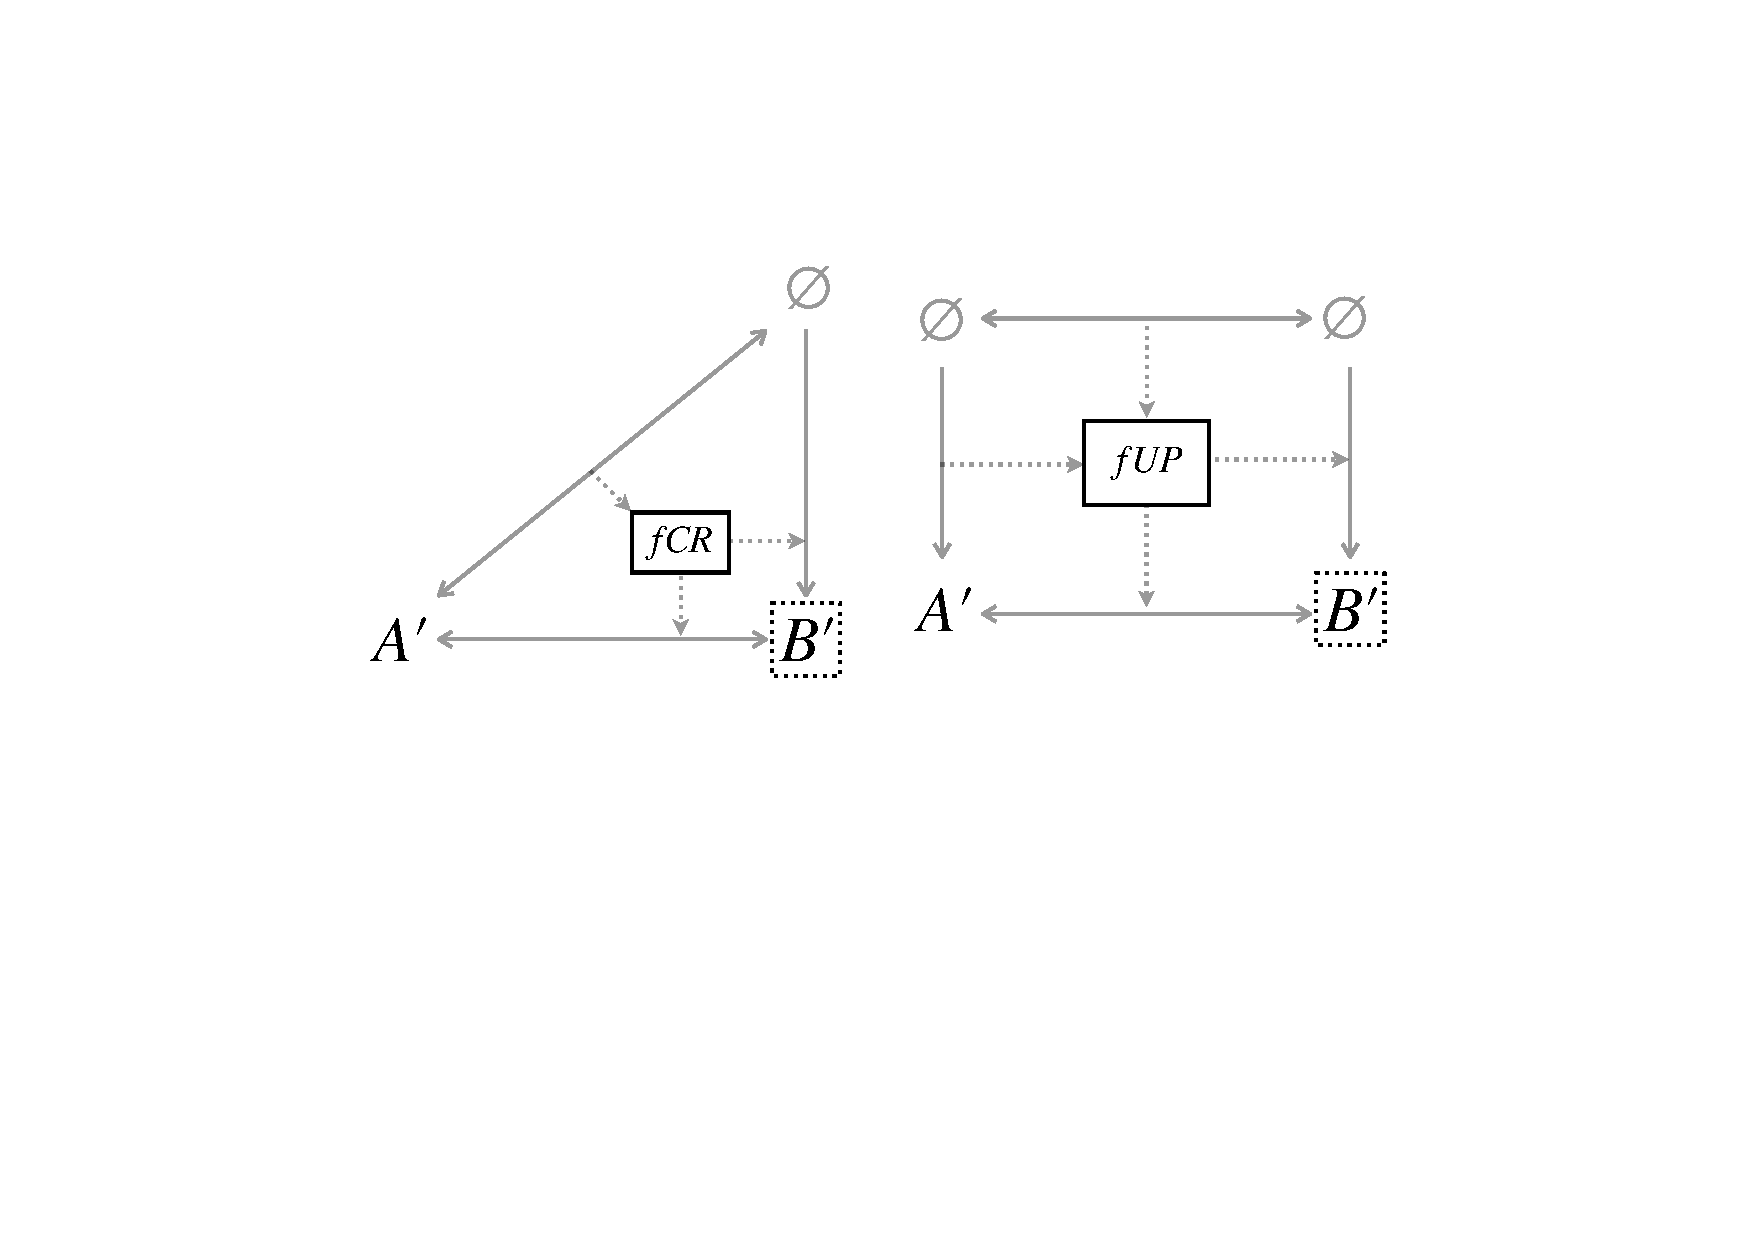
\includegraphics[width=0.8\columnwidth]{diagrams/foundations//initial-batch-based}
	\caption{Initial-batch-based Architectures}
	\label{fig:initialBatchBased}
\end{figure}
%
To apply \emph{fCR} in an initial-batch-based application scenario, the empty diag is assumed and provided as additional input to produce $\emptyset \rightarrow B'$ and $A' \leftrightarrow B'$.
In this scenario, only $B'$ is typically required as output, although a bx tool would produce a corr as well.
%
Similarly, \emph{fUP} can be applied by assuming and providing the empty corr $\emptyset \leftrightarrow \emptyset$ and $\emptyset \rightarrow A'$.
%
Note that both architectures do not require any auxiliary operations as the implied empty diag, corr, and delta are typically trivial to compute.
In practice, however, (mis)using a bx tool for this simple application scenario can be much more inefficient than a standard transformation, and we are thus not aware of any dedicated bx tool that addresses solely this applications scenario. 

Figure~\ref{fig:initialStateBased} depicts three architectures addressing the much more common bx application scenario \emph{initial-state-based}.
In this scenario, the previous output model $B$ is additionally provided as input, so that the bx tool has the chance of preserving as much information as possible in $B$ while reestablishing consistency.
%
\begin{figure}[tb!]
	\centering
	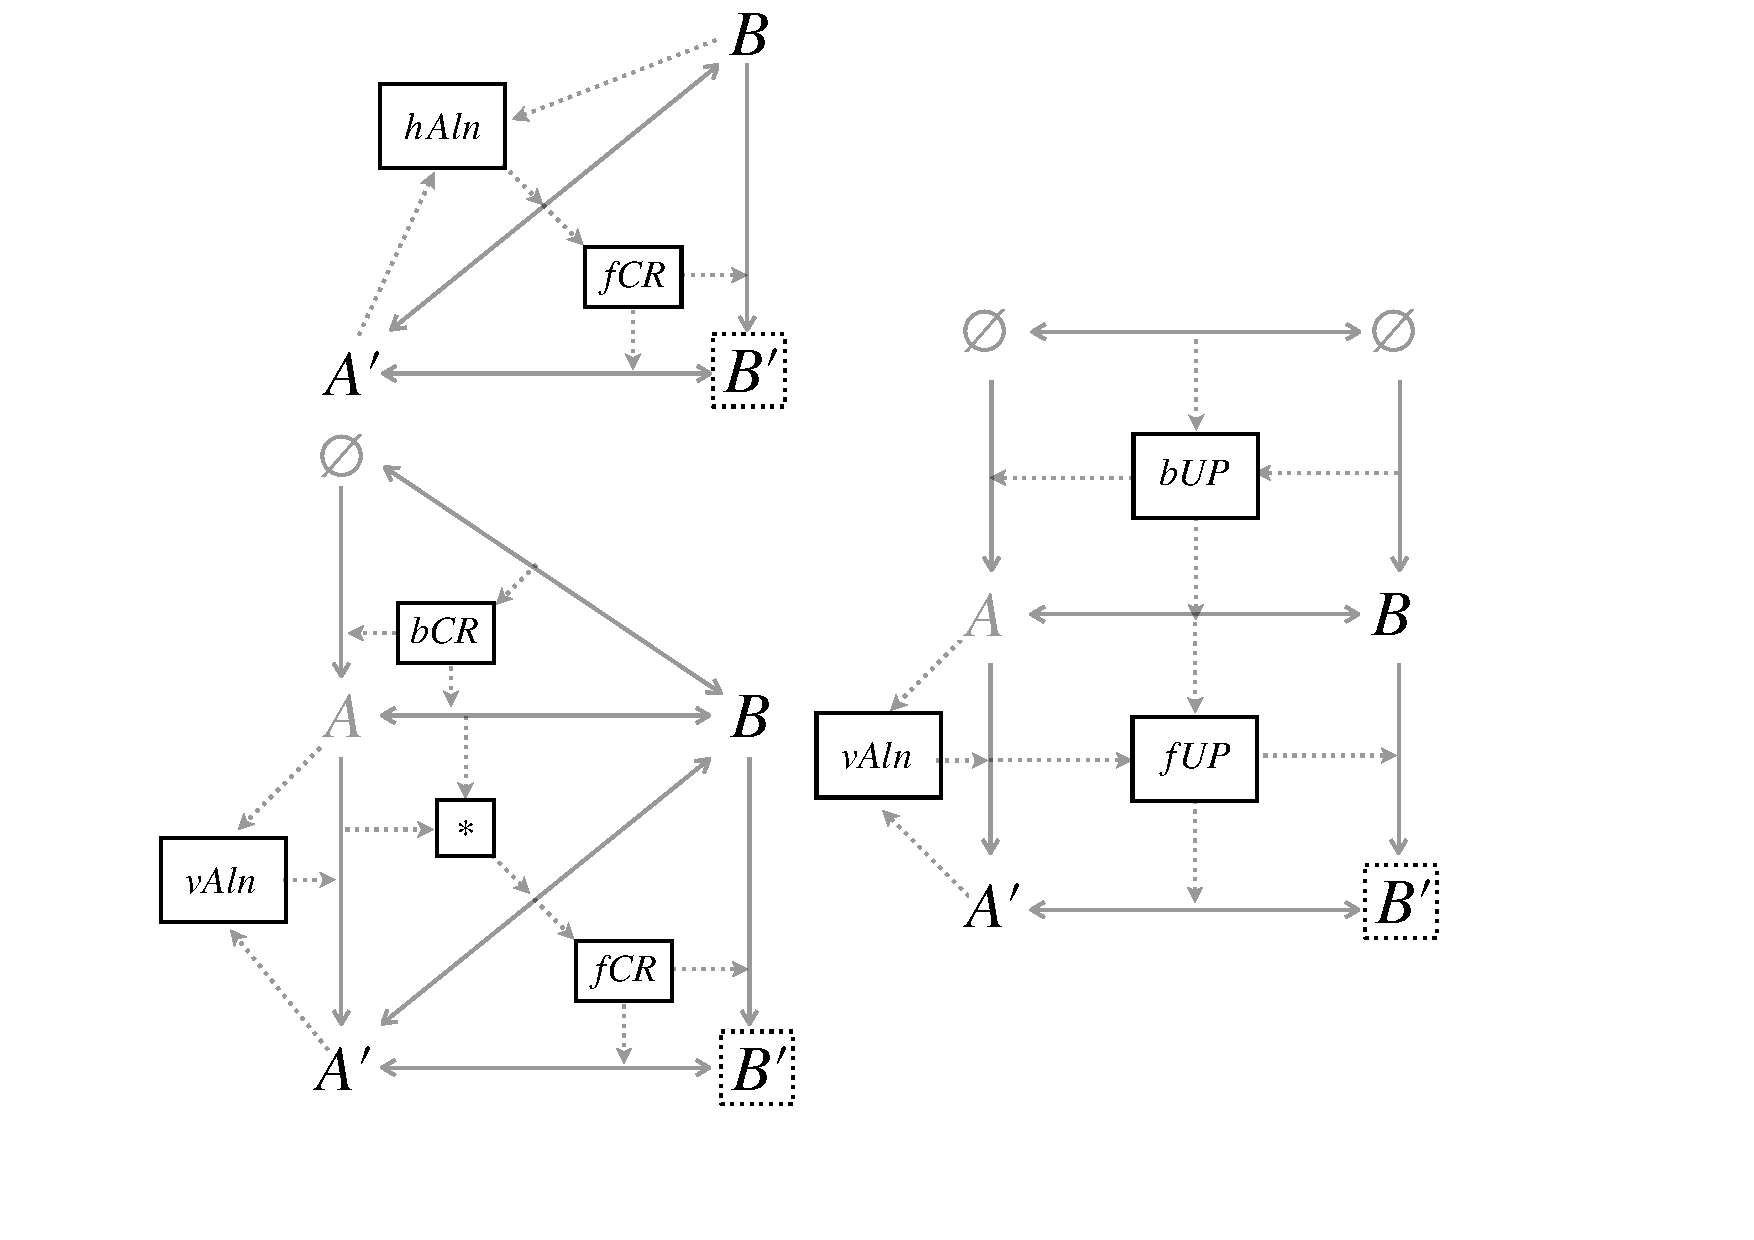
\includegraphics[width=\columnwidth]{diagrams/foundations//initial-state-based}
	\caption{Initial-state-based Architectures}
	\label{fig:initialStateBased}
\end{figure}
%
The conceptually simplest architecture makes use of \emph{fCR} by computing a diag between $A'$ and $B$ using \emph{hAln}.
%
If both \emph{bCR} and \emph{fCR} are available, \emph{vAln} can be used in place of \emph{hAln}, by first determining $A \leftrightarrow B$, then $A \rightarrow A'$ via \emph{vAln}, and then the required diag $A' \leftrightarrow B$ with $\ast$.
While this might sound much more complex, it can make sense if all necessary operations are available, while \emph{hAln} is not.
%
The propagation-based architecture for this scenario is also rather complex, requiring \emph{bUP} to determine $A \leftrightarrow B$ and \emph{vAln} to establish the require input delta $A \rightarrow A'$ for \emph{fUP}.
%
From this discussion it is clear that initial-state-based bx tools tend to favour the simpler restoration-based architecture.

Figure~\ref{fig:initialDiagBased} depicts architectures addressing the initial-diag-based application scenario.
This represents a perfect fit for a restoration-based architecture, as \emph{fCR} can be directly applied without requiring any auxiliary operations.
It is also of practical relevance, as $A$ is often destructively changed to $A$ in many application scenarios, leaving $A' \leftrightarrow B$ naturally as the left-over corr. 
Note that the typical output for this scenario is the updated, consistent corr $A' \leftrightarrow B'$.
%
\begin{figure}[tb!]
	\centering
	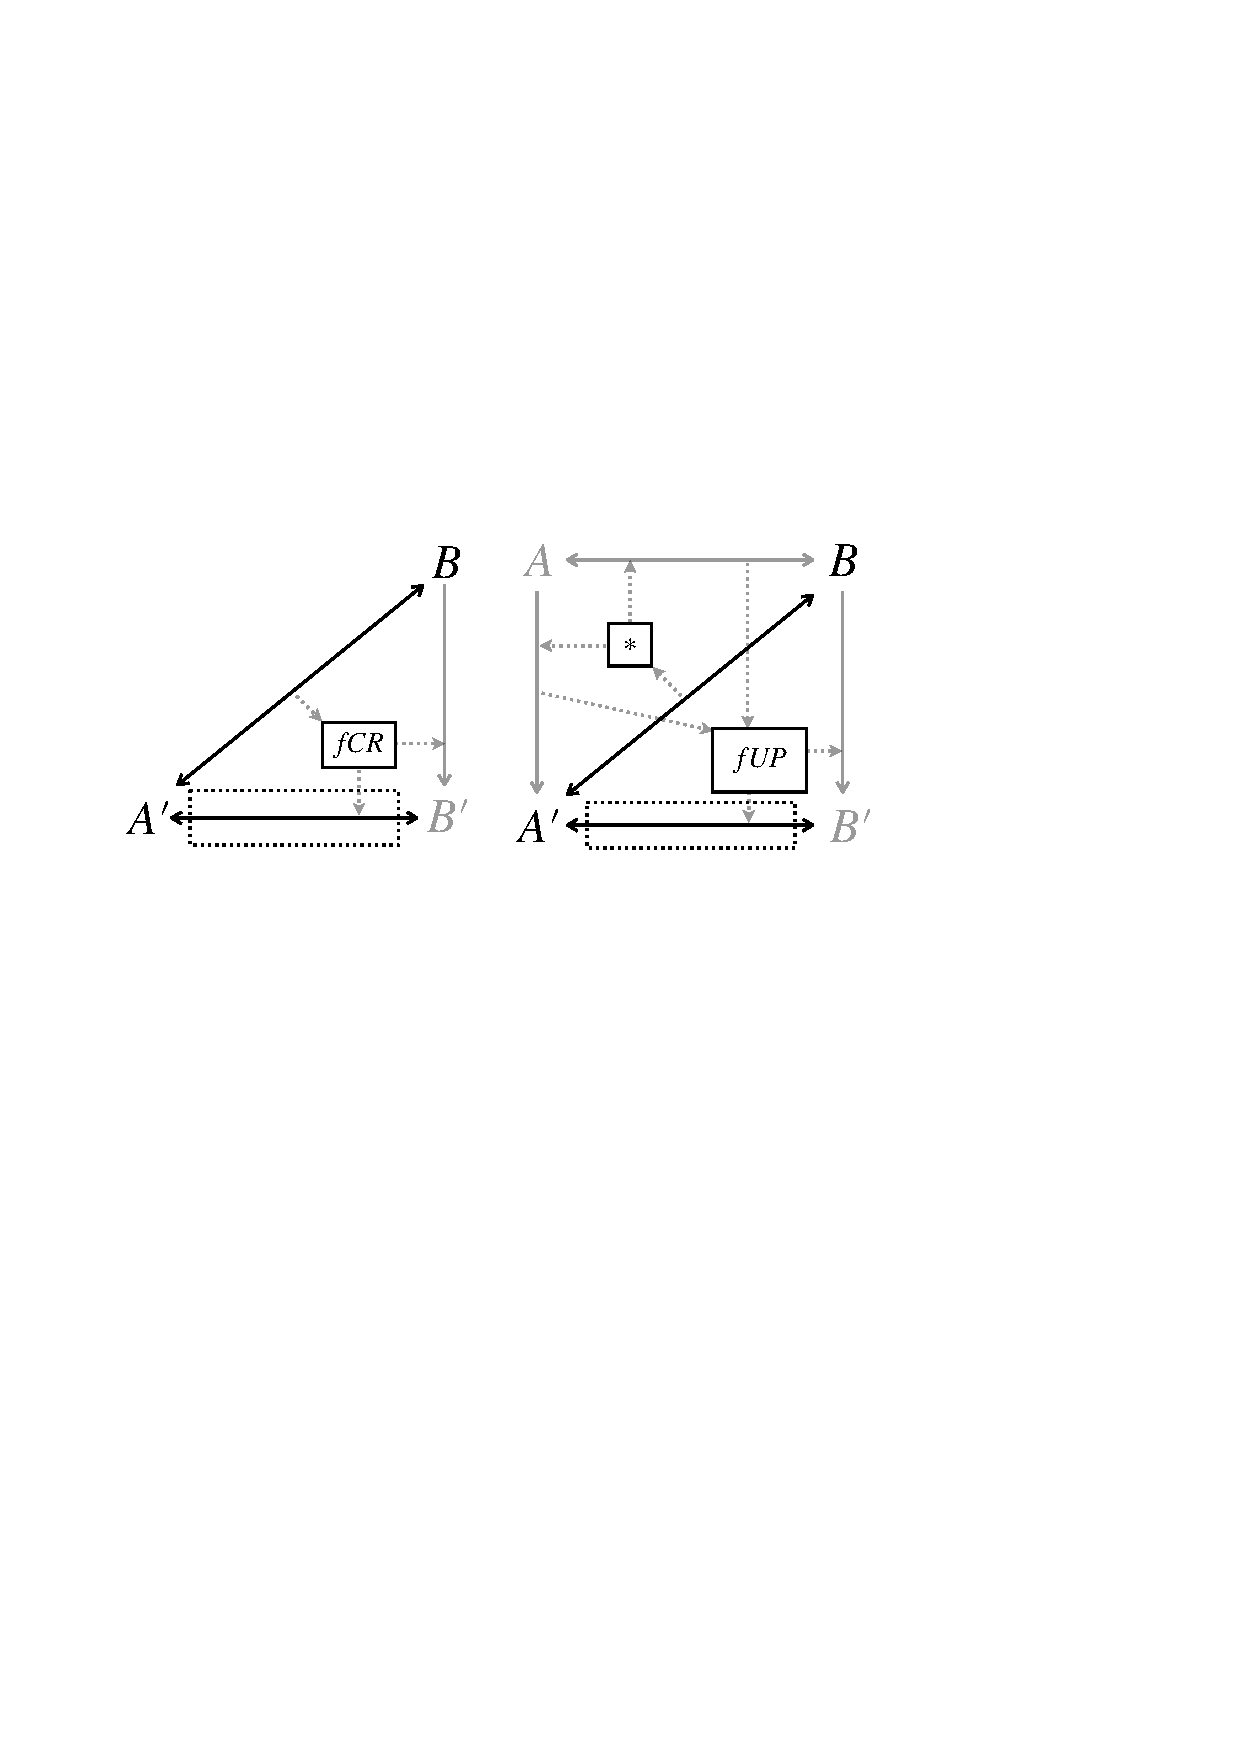
\includegraphics[width=0.755\columnwidth]{diagrams/foundations/initial-diag-based}
	\caption{Initial-diag-based Architectures}
	\label{fig:initialDiagBased}
\end{figure}
%
While it is theoretically possible to address initial-diag-based scenarios with a propagation-based architecture, Figure~\ref{fig:initialDiagBased} indicates why this is never implemented: to apply $fUP$, one would have to determine $A \rightarrow B$ and $A \rightarrow A'$ from the diag, a task  comparable in complexity to \emph{fCR/bCR}.

Figure~\ref{fig:stateBatchBased} depicts architectures addressing the state-batch-based application scenario.
In all cases, $A$ has to be extended to $A \leftrightarrow B$.
\emph{fCR} can then be used either by combining \emph{vAln} and $\ast$, or by using \emph{hAln} to directly determine $A' \leftrightarrow B$.
The propagation-based architecture uses \emph{vAln} to detemine the missing input delta for $fUP$.
%
\begin{figure}[tb!]
	\centering
	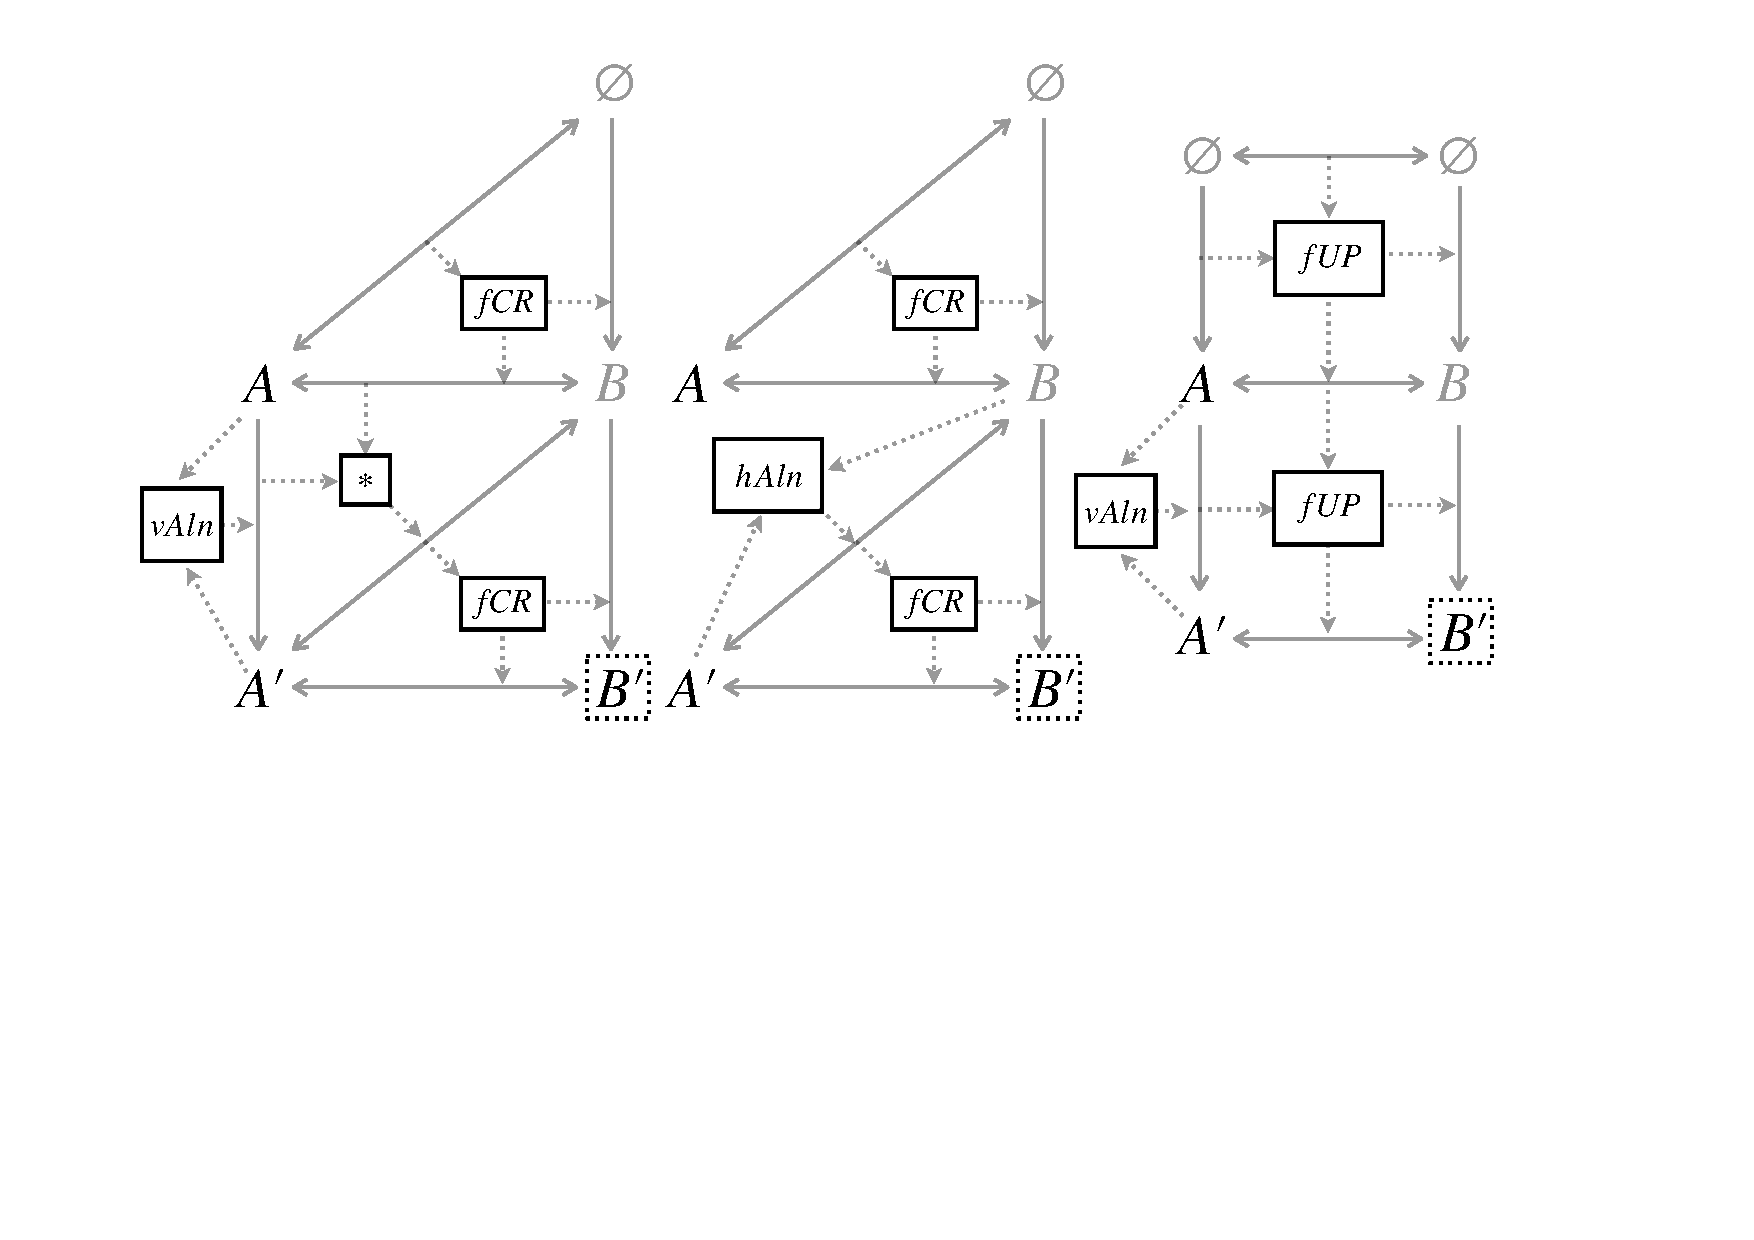
\includegraphics[width=\columnwidth]{diagrams/foundations//state-batch-based}
	\caption{State-batch-based Architectures}
	\label{fig:stateBatchBased}
\end{figure}
%
The complexity of all three architectures indicate that a state-batch-based application scenario is relatively unfavourable compared to the initial-state-based case.

Figure~\ref{fig:stateStateBased} depicts two architectures addressing the state-state-based application scenario.
In both cases both \emph{hAln} and \emph{vAln} are required to recover the corr $A \leftrightarrow B$ and input delta $A \rightarrow A'$.
While this already constitutes the input for \emph{fUP}, the restoration-based architecture additionally requires $\ast$ to detemrine the diag for \emph{fCR}.
%
\begin{figure}[tb!]
	\centering
	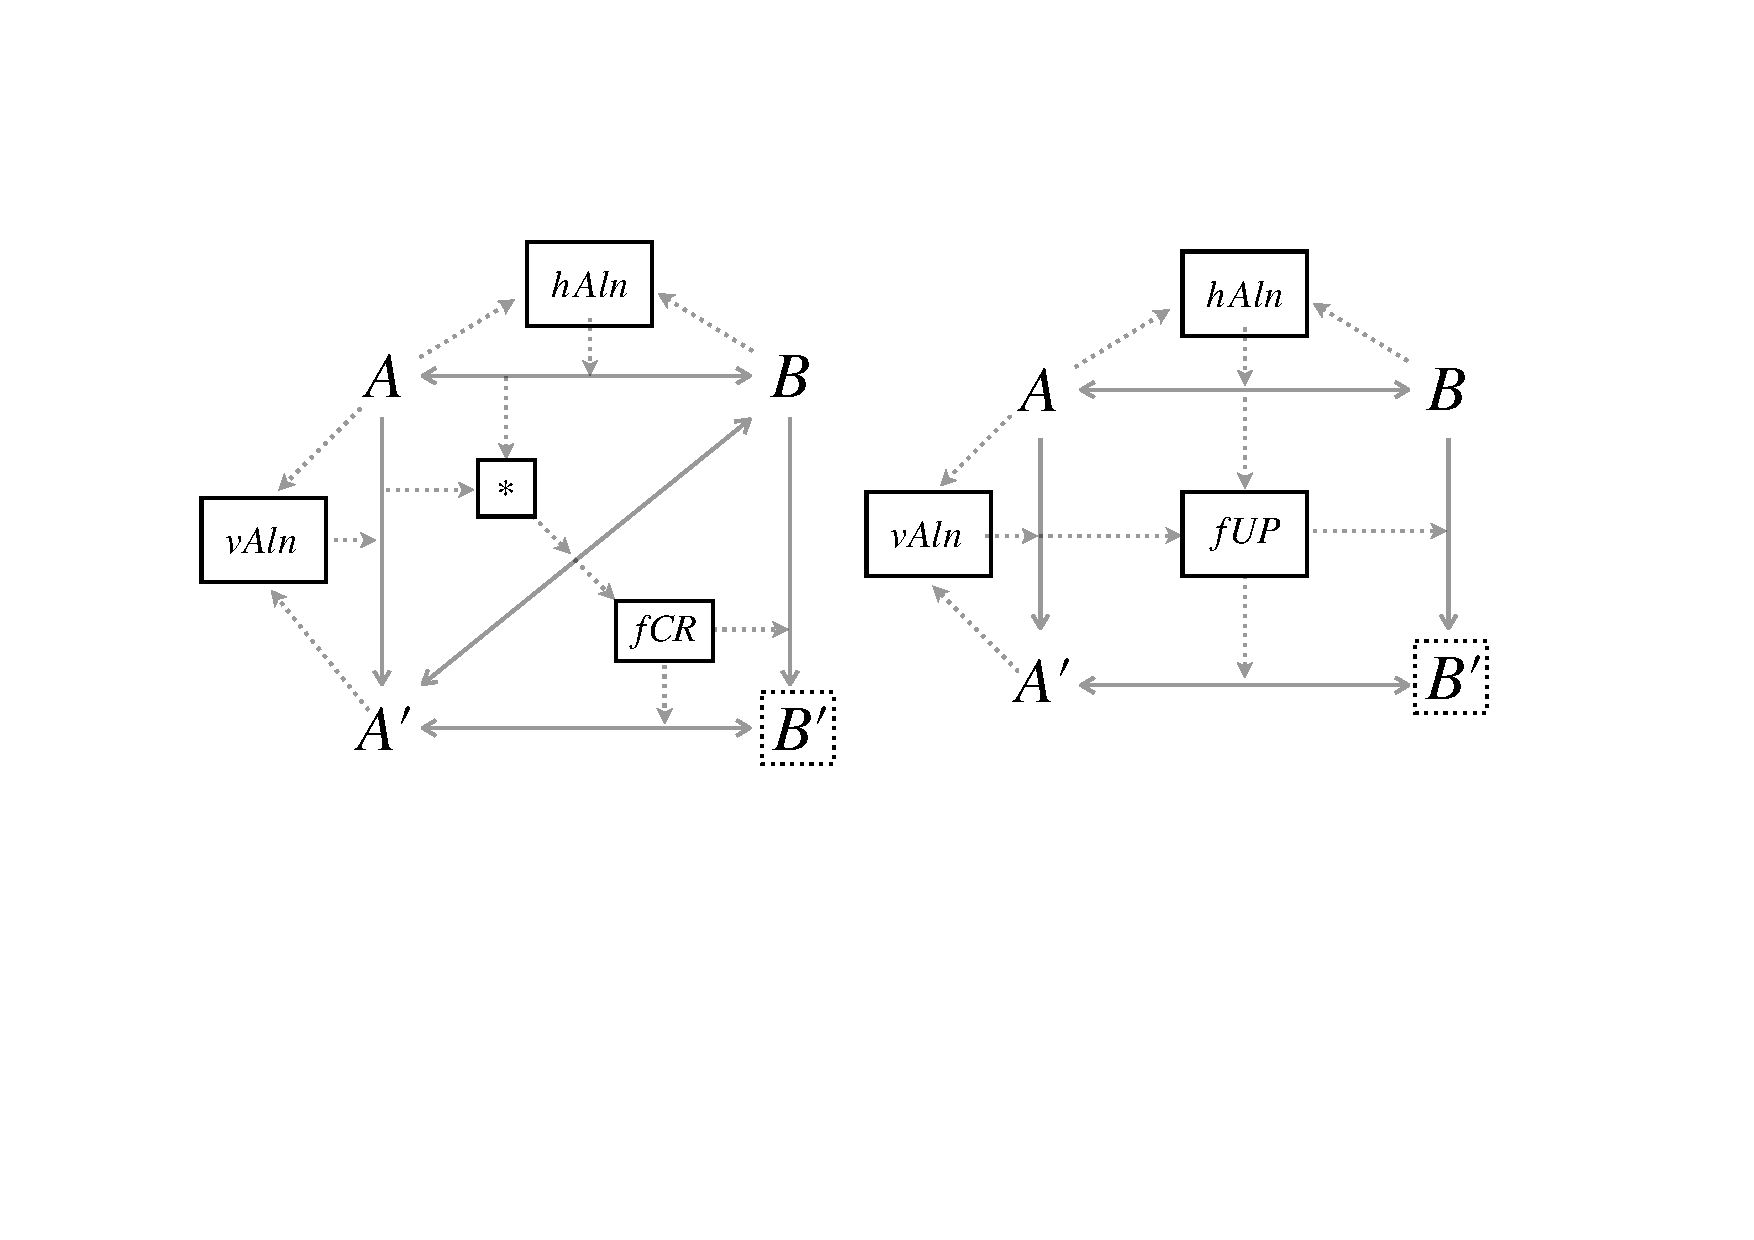
\includegraphics[width=\columnwidth]{diagrams/foundations//state-state-based}
	\caption{State-state-based Architectures}
	\label{fig:stateStateBased}
\end{figure}

The architectures depicted in Figure~\ref{fig:stateCorrBased} for the state-corr-based application scenario are fairly analogous to the state-state-based case.
The only difference and simplification is that the required corr is supplied as input and \emph{vAln} is therefore not needed.
\begin{figure}[tb!]
	\centering
	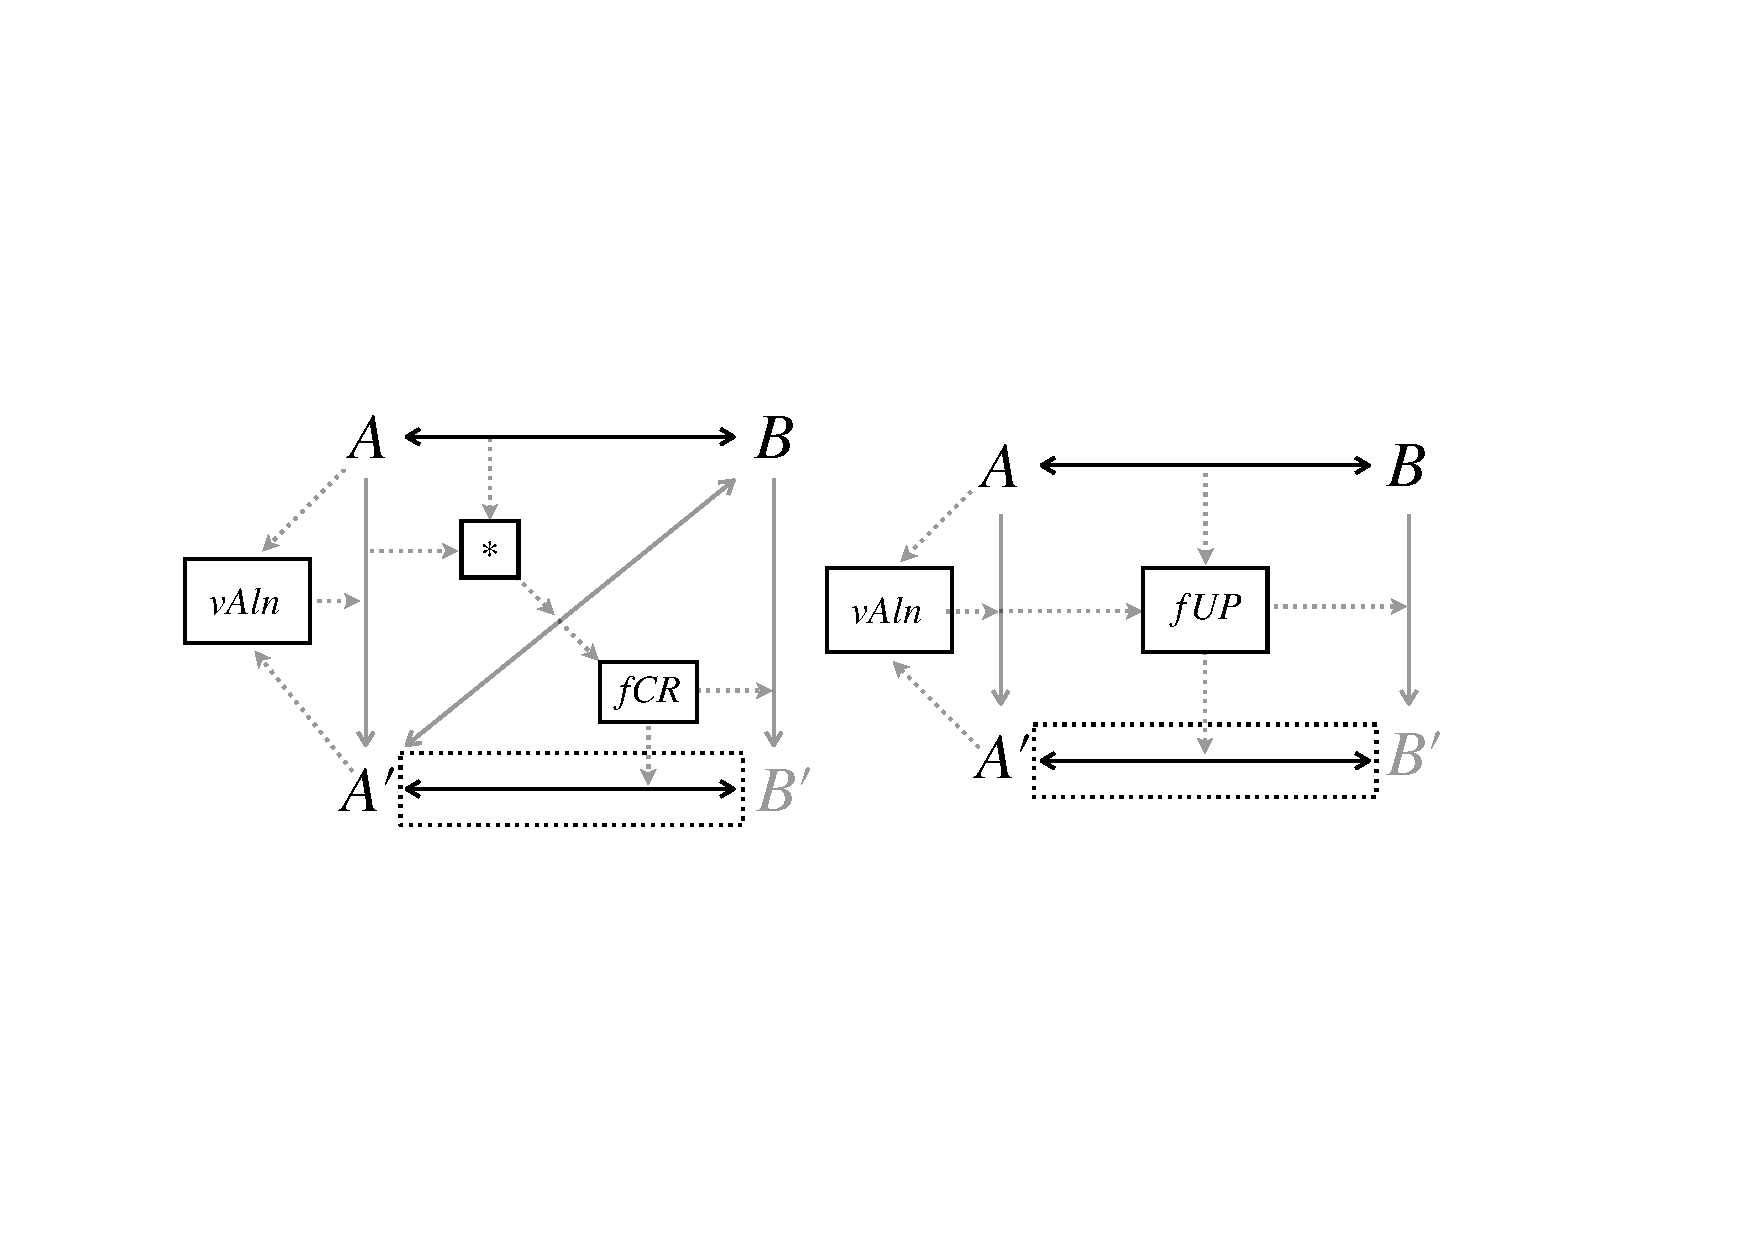
\includegraphics[width=\columnwidth]{diagrams/foundations//state-corr-based}
	\caption{State-corr-based Architectures}
	\label{fig:stateCorrBased}
\end{figure}

Figure~\ref{fig:stateAndDeltaBasedDiag} depicts architectures for state-diag-based and for delta-diag-based application scenarios.
As the required input diag for \emph{fCR} is directly supplied, providing extra input does not seem reasonable and we thus do not suggest any restoration-based architectures.
Even the propagation-based architectures appear awkward:  To make use of all provided input in the state-diag-based case, either the delta $A \rightarrow A'$ must be determined with \emph{vAln} (depicted to the left of Figure~\ref{fig:stateAndDeltaBasedDiag}), or the corr $A \leftrightarrow B$ with \emph{hAln} (not depicted in the figure).  
Taking this delta (or corr) and the supplied diag as input, $\ast$ can then be used to compute the required corr (or delta), so that \emph{fUP} can be used.
The propagation-based architecture for the delta-diag-based case is analogous, only simplified as the input delta is supplied and does not need to be computed with \emph{vAln}.
\begin{figure}[tb!]
	\centering
	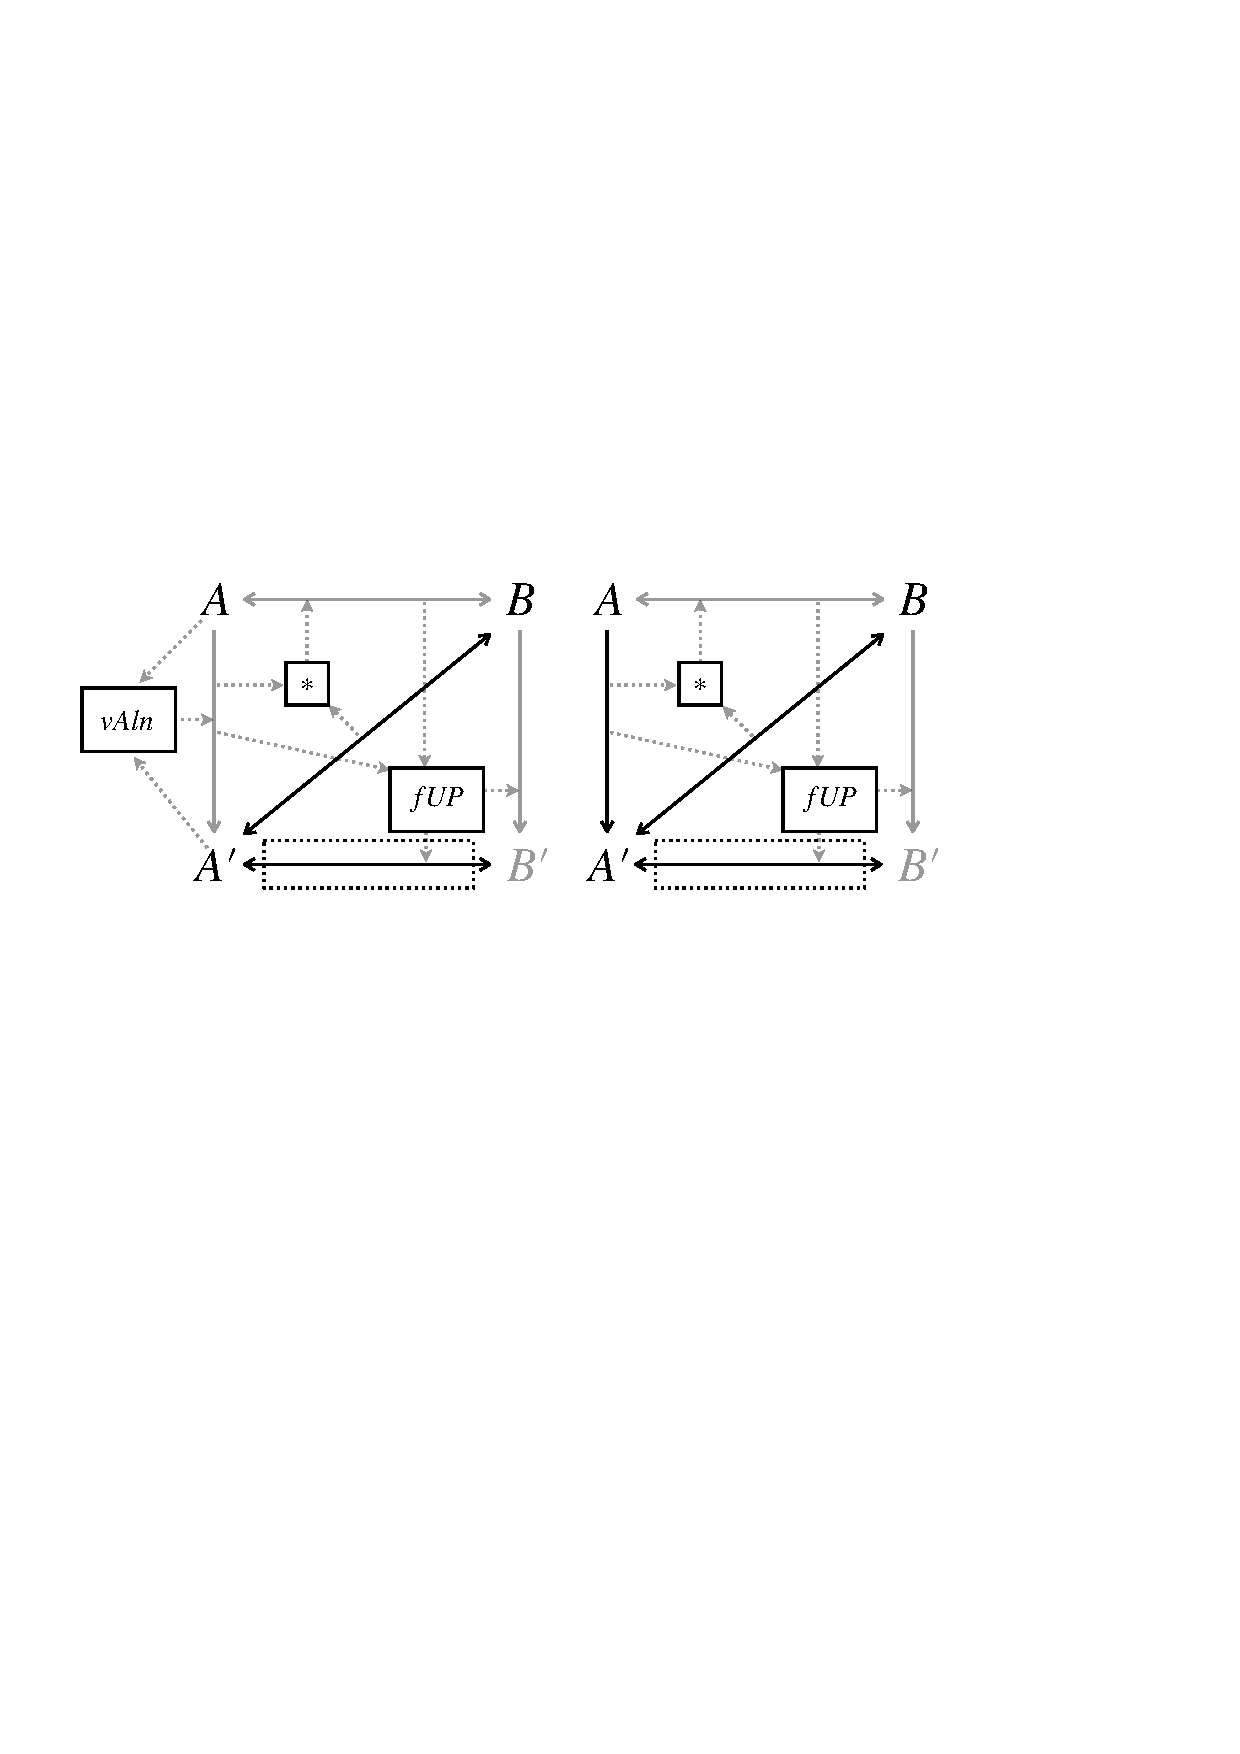
\includegraphics[width=0.82\columnwidth]{diagrams/foundations/state-and-delta-diag-based}
	\caption{State and delta-diag-based Architectures}
	\label{fig:stateAndDeltaBasedDiag}
\end{figure}

Figure~\ref{fig:deltaBatchBased} depicts the architectures for the delta-batch-based application scenario.
These are simplified versions of architectures for the state-batch-based case, as the required input delta is now provided and does not need to be computed via \emph{vAln}.
Note that both architecture neither require auxiliary alignment, nor \emph{bCR} (\emph{bUP}) for consistency restoration (update propagation).  
\begin{figure}[tb!]
	\centering
	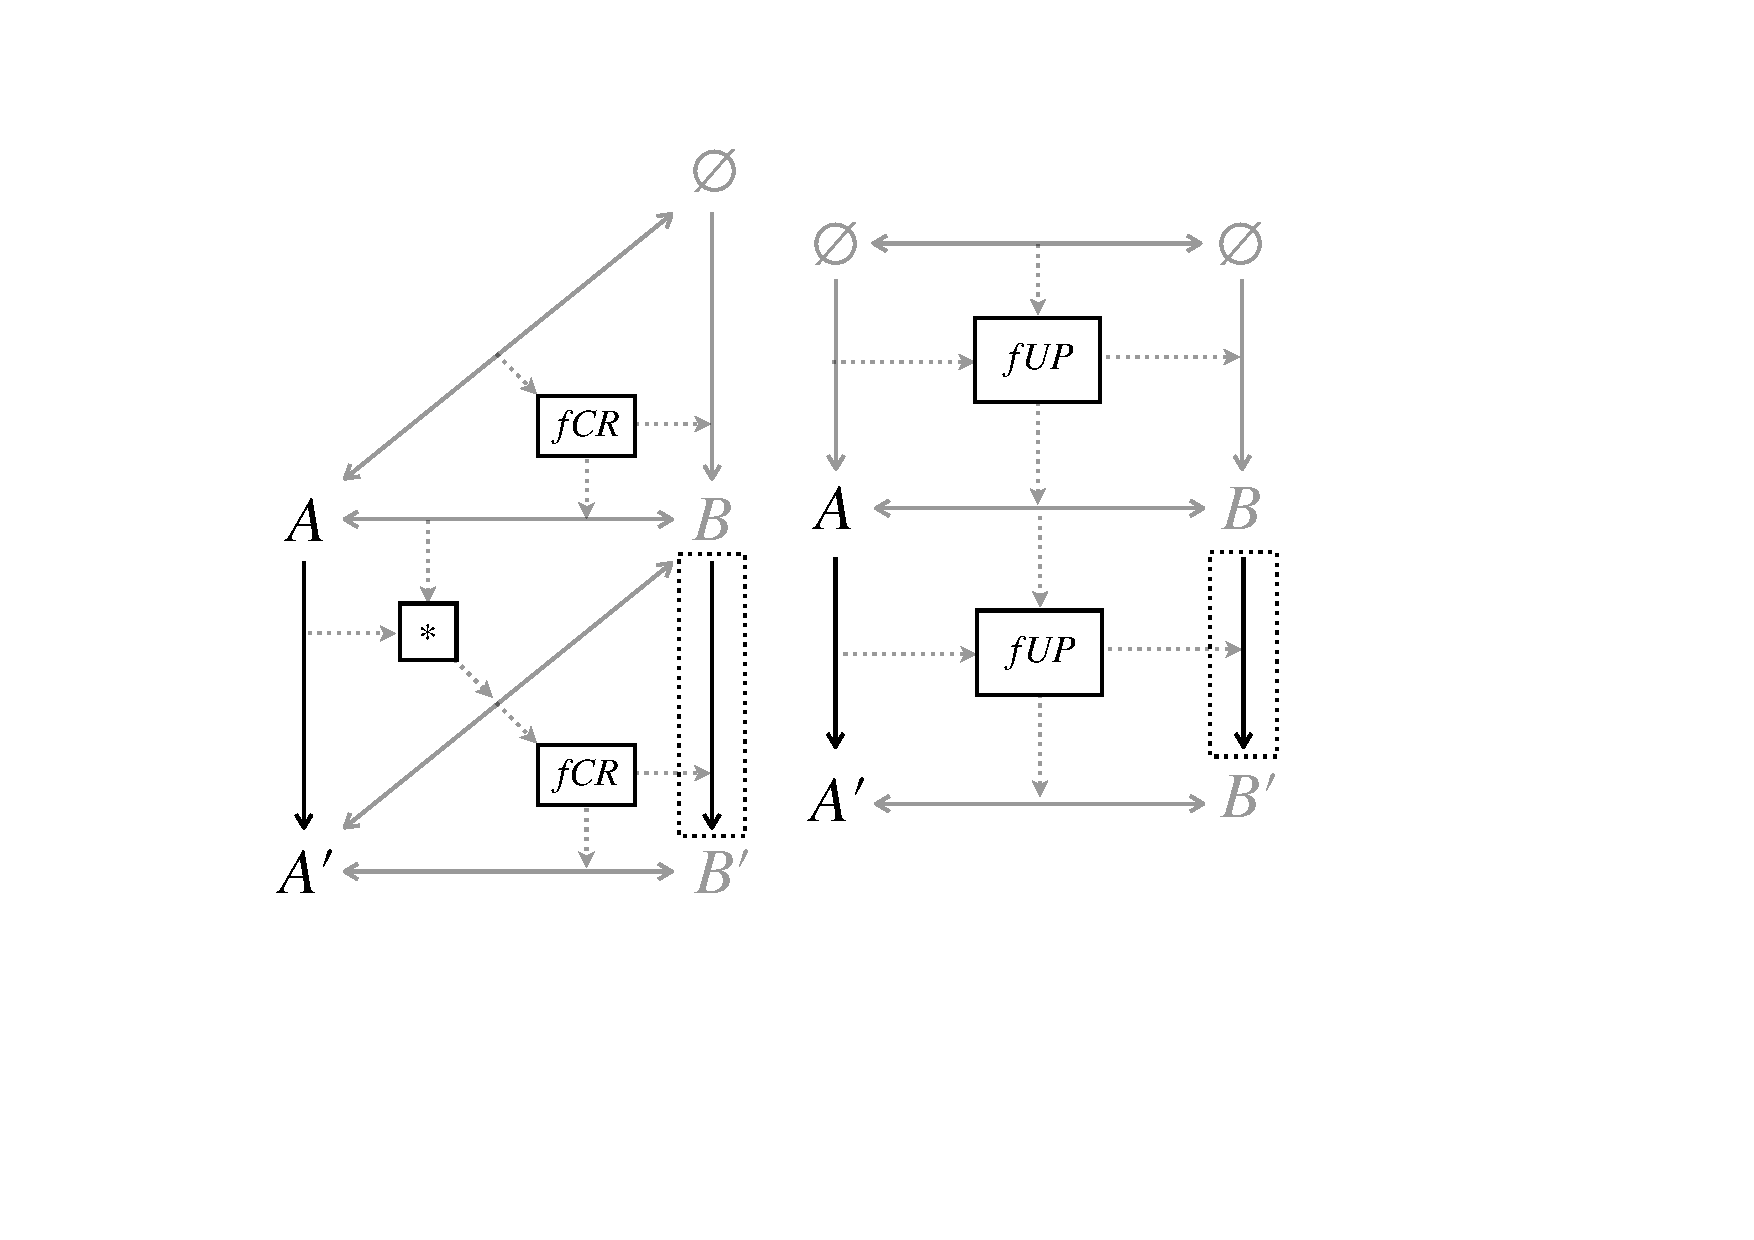
\includegraphics[width=0.73\columnwidth]{diagrams/foundations/delta-batch-based}
	\caption{Delta-batch-based Architectures}
	\label{fig:deltaBatchBased}
\end{figure}

The architectures depicted in Figure~\ref{fig:deltaStateBased} are for the delta-state-based application scenario.
As the previous target model $B$ is provided in this scenario, the architectures can use \emph{hAln} to determine the corr $A \leftrightarrow B$ and can make do without a second application of \emph{fCR} (\emph{fUP}) as in the delta-batch-based case.  
\begin{figure}[tb!]
	\centering
	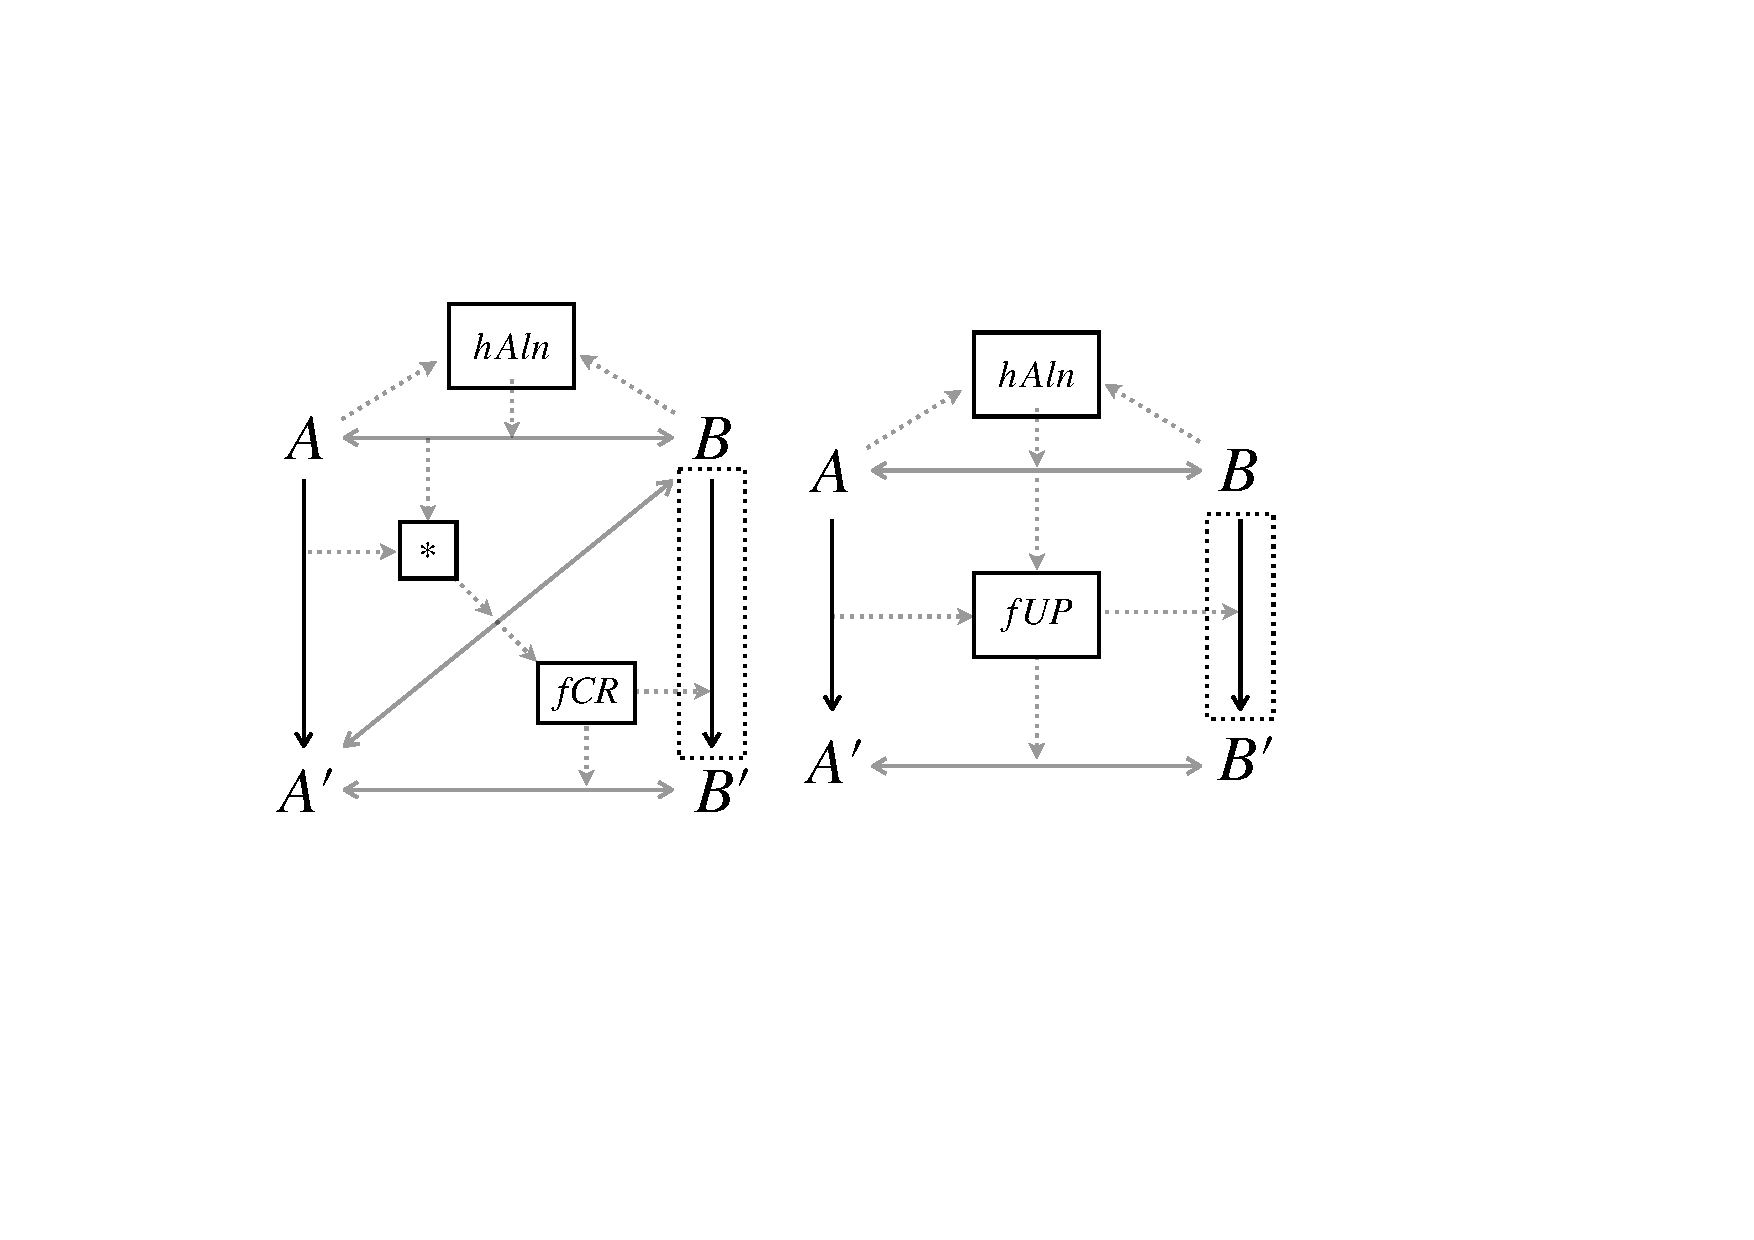
\includegraphics[width=0.75\columnwidth]{diagrams/foundations/delta-state-based}
	\caption{Delta-state-based Architectures}
	\label{fig:deltaStateBased}
\end{figure}

Finally, Figure~\ref{fig:deltaCorrBased} depicts the architectures for the delta-corr-based application scenario.
The diagrams indicate that this is the ideal case for applying $fUP$ as exactly what is required is available as input.
The restoration-based architecture only requires realignment via $\ast$, which is usually a simple operation in this case.
\begin{figure}[tb!]
	\centering
	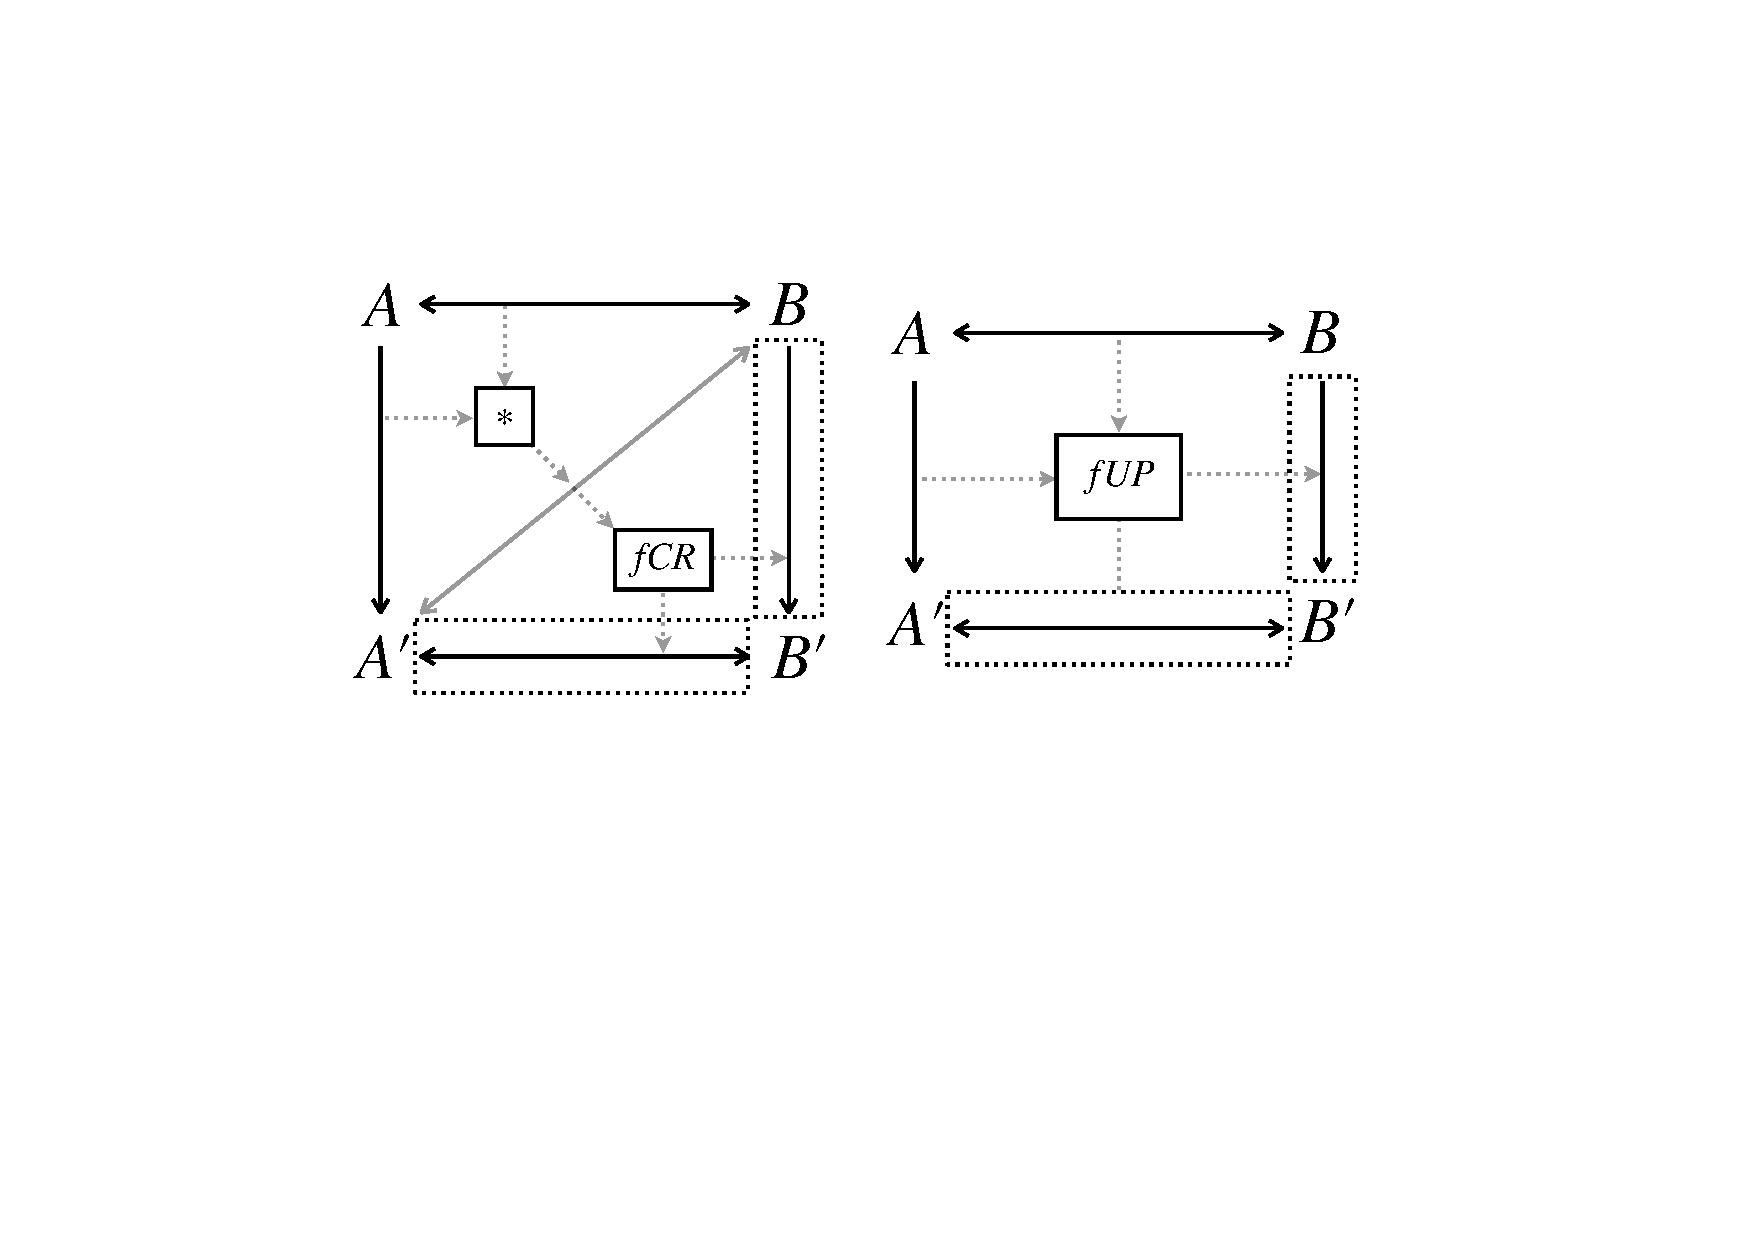
\includegraphics[width=0.75\columnwidth]{diagrams/foundations/delta-corr-based}
	\caption{Delta-corr-based Architectures}
	\label{fig:deltaCorrBased}
\end{figure}

% Summary?
As a summary based on the discussion of all architectures, Figure~\ref{fig:evalOfApplicationScenarios} depicts the grid of all 11 feasible application scenarios, now color-coded to indicate the simplicity of the corresponding bx tool architectures required to address each case.
Each cell in the grid is additionally divided with a vertical line ($~|~$), with labels to the left (restoration-based architectures) and to the right (propagation-based architectures) consisting of plus and minus symbols corresponding to the color.
\begin{figure}[tb!]
	\centering
	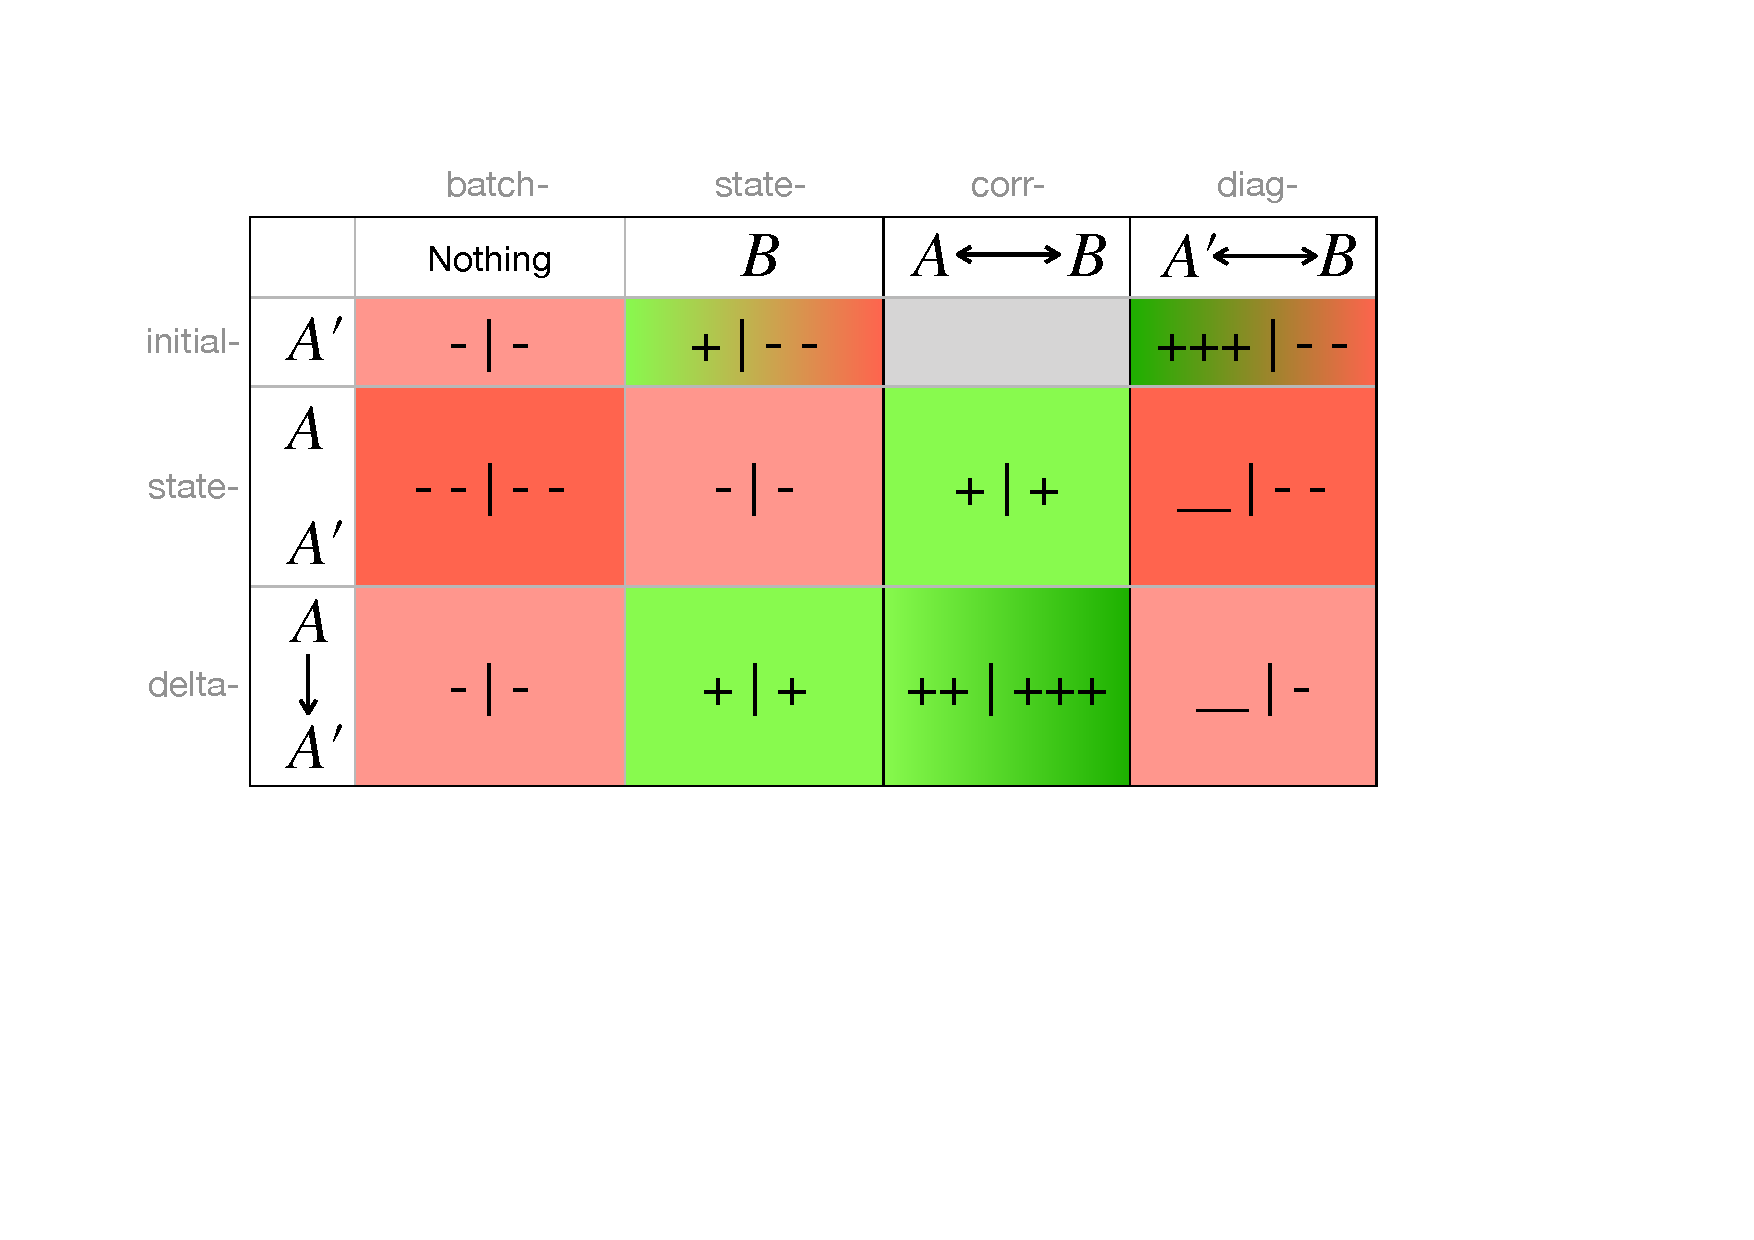
\includegraphics[width=0.9\columnwidth]{diagrams/foundations/EvalOfApplicationScenarios.pdf}
	\caption{Architecture-based evaluation of scenarios}
	\label{fig:evalOfApplicationScenarios}
\end{figure}
Plus symbols (green) indicate a simple, minus symbols (red) a complicated bx tool architecture.  

\begin{figure*}[tb!]
	\centering
	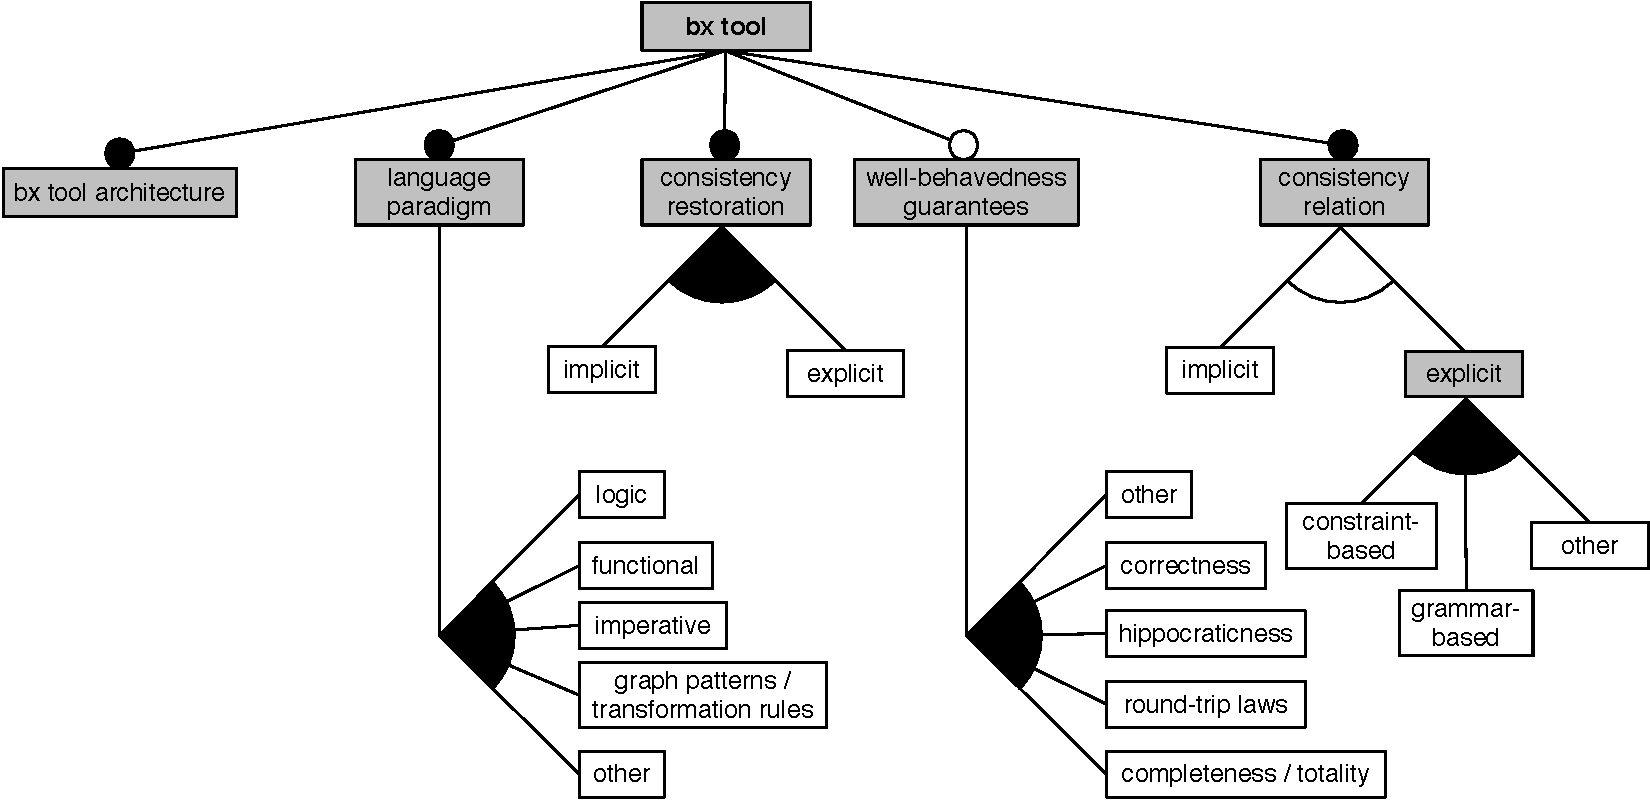
\includegraphics[width=\textwidth]{diagrams/foundations/feature-model-bx-tool}
	\caption{Bx tool variability as a feature model}
	\label{fig:featureModelBxTools}
\end{figure*}

\subsection{Classifying BX Tools}
\label{sec:classifying-bx-tools}
Reflecting the 11 application scenarios and possible bx tool architectures discussed in detail in previous paragraphs, the variability of bx tool architectures is represented as a feature model in Figure~\ref{fig:featureModelBxTools}, extended to cover some additional features of bx tools.
Our goal in this paper is not to suggest a further exhaustive feature model for bx approaches such as Hidaka et al.~\cite{SOSYM-Hidaka2016}, but more to make intensive use of a minimal set of core features to classify the different bx tools used to solve our bx benchmark.

Using standard feature model notation, features are denoted as rectangles; a grey fill denotes \emph{abstract} features that are only used to group other features.
Circles with a black fill indicate mandatory children, circles without a fill optional children.
Children connected with an angle without a fill are exclusively ored, while children connected with an angle with a black fill are ored.
Features that exclude each other are connected with a dashed, double-headed (red) arrow.

%%%% Rewrite

A bx tool must have a bx tool architecture, developed in a specific style (either restoration-based using \emph{fCR/bCR} or propagation-based using \emph{fUP/bUP}), and addressing a specific application scenario according to expected input. 
%
Concerning horizontal input, a scenario can exclusively require no input at all (batch), the previous output model (state-based), a diag (diag-based), or a corr (corr-based) as input.
%
In contrast, vertical input is a mandatory feature, forcing an exclusive choice between requiring just the input model (initial-based), the previous and changed input models (state-based), and an input delta  (delta-based).
In practice, it is also informative to know if a bx tool expects an s-delta or o-delta.
Finally, as explained previously, requiring a corr and only the input model (initial) is contradictory, hence the exclusion between these two features.

The core feature of a bx tools is consistency maintenance and we have observed that this can be either \emph{implicit}, e.g., based on the underlying consistency relation and some governing laws the bx tool automatically derives \emph{fCR/bCR} or \emph{fUP/bUP} as required, or \emph{explicit}, e.g., the bx tool requires implementations of \emph{fCR/bCR} or \emph{fUP/bUP}, but performs for instance some checking for compatibility of these implementations.
Some bx tools allow a mixture of implicit and explicit, e.g., requiring an implementation of \emph{fCR} (\emph{fUP}) and automatically deriving a compatible \emph{bCR} (\emph{bUP}), or vice-versa.

A major goal of bx languages and tools is often to provide some added value compared to implementing consistency maintenance using standard unidirectional transformation languages.
While this goal can be realized as an attempt to increase productivity, it is often also realized as an attempt to increase the \emph{quality} of implemented synchronization solutions.
In Figure~\ref{fig:featureModelBxTools}, therefore, we include an optional feature \emph{well-behavedness guarantees}, which can include a combination of correctness, hippocraticness, round-trip laws, and completeness (totality) guarantees.
All mentioned guarantees apart from the last two have been informally introduced in Section~\ref{sec:FamiliesToPersons}; termination is self explanatory.
Consistency restoration (update propagation) is \emph{complete} if \emph{fCR} (\emph{fUP}) is total on a  (preferably statically) well-defined domain, i.e., for a well-defined subset of input deltas and corrs/diags in the triple space for consistency maintenance.

% Mandatory:  Consistency relation
The final, mandatory feature of a bx tool is its underlying \emph{consistency relation}.
This has to be specified in some manner, either \emph{implicitly}, e.g., by providing implementations of \emph{fCR/bCR} (\emph{fUP/bUP}) together with round-trip laws, or \emph{explicitly}, by specifying a set of constraints, providing a grammar (language membership as consistency check), implementing a consistency checker in some suitable (programming) language, or via a combination of these (partial) specifications, e.g., grammar-based for structural parts of the model and constraint-based for attribute values.